\documentclass{article}

% Recommended, but optional, packages for figures and better typesetting:
\usepackage{microtype}
\usepackage{graphicx}
\usepackage{subfigure}
\usepackage{booktabs} % for professional tables

% hyperref makes hyperlinks in the resulting PDF.
% If your build breaks (sometimes temporarily if a hyperlink spans a page)
% please comment out the following usepackage line and replace
% \usepackage{icml2023} with \usepackage[nohyperref]{icml2023} above.
\usepackage{hyperref}


% Attempt to make hyperref and algorithmic work together better:
\newcommand{\theHalgorithm}{\arabic{algorithm}}
\newcommand{\Scomment}[1]  {{\bfseries \color{red} S:#1}}
% Use the following line for the initial blind version submitted for review:
\usepackage[accepted]{icml2023}

% If accepted, instead use the following line for the camera-ready submission:
%\usepackage[accepted]{icml2023}

% For theorems and such
\usepackage{amsmath}
\usepackage{amssymb}
\usepackage{mathtools}
\usepackage{amsthm}
%\usepackage{multirow}

% if you use cleveref..
\usepackage[capitalize,noabbrev]{cleveref}

%%%%%%%%%%%%%%%%%%%%%%%%%%%%%%%%
% THEOREMS
%%%%%%%%%%%%%%%%%%%%%%%%%%%%%%%%
\theoremstyle{plain}
\newtheorem{theorem}{Theorem}[section]
\newtheorem{proposition}[theorem]{Proposition}
\newtheorem{lemma}[theorem]{Lemma}
\newtheorem{corollary}[theorem]{Corollary}
\theoremstyle{definition}
\newtheorem{definition}[theorem]{Definition}
\newtheorem{assumption}[theorem]{Assumption}
\theoremstyle{remark}
\newtheorem{remark}[theorem]{Remark}

% Todonotes is useful during development; simply uncomment the next line
%    and comment out the line below the next line to turn off comments
%\usepackage[disable,textsize=tiny]{todonotes}
\usepackage[textsize=tiny]{todonotes}


% The \icmltitle you define below is probably too long as a header.
% Therefore, a short form for the running title is supplied here:
\icmltitlerunning{Closure Discovery for Coarse-Grained PDEs using Multi-Agent Reinforcement Learning }

\begin{document}

\twocolumn[
\icmltitle{Closure Discovery for Coarse-Grained Partial Differential Equations \\ using Multi-Agent Reinforcement Learning}

% It is OKAY to include author information, even for blind
% submissions: the style file will automatically remove it for you
% unless you've provided the [accepted] option to the icml2023
% package.

% List of affiliations: The first argument should be a (short)
% identifier you will use later to specify author affiliations
% Academic affiliations should list Department, University, City, Region, Country
% Industry affiliations should list Company, City, Region, Country

% You can specify symbols, otherwise they are numbered in order.
% Ideally, you should not use this facility. Affiliations will be numbered
% in order of appearance and this is the preferred way.
\icmlsetsymbol{equal}{*}

\begin{icmlauthorlist}
\icmlauthor{Jan-Philipp von Bassewitz}{xx,yyy}
\icmlauthor{Sebastian Kaltenbach}{xx,yyy}
\icmlauthor{Petros Koumoutsakos}{yyy}
\end{icmlauthorlist}

\icmlaffiliation{xx}{ETH Zurich, Switzerland}
\icmlaffiliation{yyy}{Harvard SEAS, United States}

\icmlcorrespondingauthor{Petros Koumoutsakos}{petros@seas.harvard.edu}

% You may provide any keywords that you
% find helpful for describing your paper; these are used to populate
% the "keywords" metadata in the PDF but will not be shown in the document
\icmlkeywords{Multi-Agent Reinforcement Learning, Closure Modeling, Partial Differential Equations, Coarse-Graining}

\vskip 0.3in
]

% this must go after the closing bracket ] following \twocolumn[ ...

% This command actually creates the footnote in the first column
% listing the affiliations and the copyright notice.
% The command takes one argument, which is text to display at the start of the footnote.
% The \icmlEqualContribution command is standard text for equal contribution.
% Remove it (just {}) if you do not need this facility.

\printAffiliationsAndNotice{}  % leave blank if no need to mention equal contribution
%\printAffiliationsAndNotice{\icmlEqualContribution} % otherwise use the standard text.

\begin{abstract}
Reliable predictions of critical phenomena, such as weather, wildfires and  epidemics are often founded on models described by Partial Differential Equations (PDEs). However, simulations that capture the full range of spatio-temporal scales in such PDEs are often prohibitively expensive. Consequently, coarse-grained simulations that employ heuristics and empirical closure terms are frequently utilized as an alternative. We propose a novel and systematic approach for identifying closures in under-resolved PDEs using Multi-Agent Reinforcement Learning (MARL). The MARL formulation incorporates inductive bias and exploits locality by deploying a central policy represented efficiently by Convolutional Neural Networks (CNN). We demonstrate the capabilities and limitations of MARL through numerical solutions of the advection equation and the Burgers' equation. Our results show accurate predictions for in- and out-of-distribution test cases as well as a significant speedup compared to resolving all scales.
\end{abstract}

\section{Introduction}
Simulations of critical phenomena such as climate,  ocean dynamics and epidemics, have become essential for decision-making, and their veracity, reliability, and energy demands have great impact on our society. Many of these simulations are based on models described by PDEs expressing system dynamics that span multiple spatio-temporal scales. Examples include  turbulence~\cite{wilcox1988multiscale}, neuroscience~\cite{dura2019netpyne}, climate~\cite{climatenas} and  ocean dynamics~\cite{mahadevan2016impact}. Today, we benefit from decades of remarkable efforts in the development of  numerical methods, algorithms, software, and hardware and witness simulation frontiers that were unimaginable even a few years ago \cite{hey2009fourth}. 
Large-scale simulations that predict the system's dynamics may use trillions of computational elements\cite{rossinelli2013a} to resolve all spatio-temporal scales, but these often address only idealized systems and their computational cost prevents experimentation and uncertainty quantification.  On the other hand, reduced order and coarse-grained models are fast, but limited by the linearization of complex system dynamics  while  their associated closures are often based on heuristics \cite{peng2021multiscale}.
 
We propose to complement coarse-grained simulations with closures in the form of a policies that are discovered by a multi-agent reinforcement learning framework. A central policy that is based on CNNs and uses locality as inductive bias,  corrects the error of the numerical discretization and improves the overall accuracy. This approach is inspired by recent work in Reinforcement Learning (RL) for image reconstruction \cite{cv_pixel_rl}. The agents learn and act locally on the grid, in a manner that is reminiscent of the numerical discretizations of PDEs based on Taylor series approximations. Hence, each agent only gets information from its spatial neighborhood. Together with a central policy, this results in efficient training, as each agent needs to process only a limited amount of observations. After training, the framework is capable of accurate predictions in both in- and out-of-distribution test cases. We remark  that the actions taken by the agents are highly correlated with the numerical errors and can be viewed as an implicit correction to the effective convolution performed via  the coarse-grained discretization of the  PDEs \cite{bergdorf2005multilevel}.  \\

\section{Related Work}
The main contribution of this work is a MARL algorithm for the discovery of closures for coarse-grained PDEs. The algorithm provides an automated process for the correction of the errors of the associated numerical discretization. We  show that the proposed method is able to capture scales beyond the training regime and provides a potent method for solving PDEs with high accuracy and limited resolution.
\newpage
\textbf{Machine Learning and Partial Differential Equations:}
In recent years, there has been significant interest in learning the solution of PDEs using Neural Networks. Techniques such as 
PINNs \cite{raissi2019physics,karniadakis2021physics}, DeepONet \cite{lu2021learning}, the Fourier Neural Operator \cite{li2020fourier}, NOMAD \cite{seidman2022nomad}, Clifford Neural Layers \cite{brandstetter2022clifford} and an invertible formulation \cite{kaltenbach2023semi} have shown promising results for both forward and inverse problems. However, there are concerns about their accuracy and related computational cost, especially for low-dimensional problems \cite{karnakov2022optimizing}. These methods aim to substitute numerical discretizations with neural nets, in contrast to our RL framework, which aims to complement them. Moreover, their loss function is required to be differentiable, which is not necessary for the stochastic formulation of the RL reward.

\textbf{Reinforcement Learning:}
Our work is based upon recent advances in RL \cite{sutton2018reinforcement} including  PPO \cite{ppo} and the Remember and Forget Experience Replay (ReFER) algorithm \cite{novati2019}. It is  related to other methods that employ multi-agent learning \cite{novati2021automating,albrecht2023multi, wen2022multi,bae2022scientific,yang2020overview} for closures except that here we use as reward not global data (such as energy spectrum) but the local dicsretization error as quantified by fine-grained simulations. The present approach is designed to solve various PDEs using a central policy and it is related to similar work for  image reconstruction \cite{cv_pixel_rl}. We train a central policy for all agents in contrast to other methods where agents are trained on  decoupled subproblems \cite{freed2021learning, albrecht2023multi, sutton2023reward}. 

\textbf{Closure Modeling:}
The development of machine learning methods for discovering closures for under-resolved  PDEs has gained attention in recent years. Current approaches are mostly tailored to specific applications such as turbulence modeling \cite{ling2016reynolds, durbin2018some,novati2021automating,bae2022scientific} and use data such as energy spectra and drag coefficients of the flow in order to train the RL policies. In \cite{lippe2023pde}, a more general framework based on diffusion models is used to improve the solutions of Neural Operators for temporal problems using a multi-step refinement process. Their training is based on supervised learning in contrast to the present RL approach which additionally complements existing numerical methods instead of neural network based surrogates \cite{li2020fourier,gupta2022towards}.

\textbf{Inductive Bias:}  
The incorporation of  prior knowledge regarding the physical processes described by the PDEs, into machine learning algorithms is critical for their training in the Small Data regime and for increasing the accuracy during extrapolative predictions \cite{goyal2022inductive}. One way to achieve this is by shaping appropriately the loss function \cite{karniadakis2021physics, kaltenbach2020incorporating,yin2021augmenting, wang2021learning, wang2022respecting}, or by incorporating parameterized mappings that are based on known constraints \cite{greydanus2019hamiltonian,kaltenbach2021physics, cranmer2020lagrangian}. Our RL framework incorporates locality and is thus consistent with numerical discretizations that rely on local Taylor series based approximations. The incorporation of  inductive bias in RL has also been attempted by focusing on the beginning of the training phase \cite{uchendu2023jump,walke2023don} in order to shorten the exploration phase.

\section{Methodology}
We consider a time-dependent, parametric, non-linear PDE defined on a regular domain $\Omega$. The solution of the PDE depends on its initial conditions (ICs) as well as its input parameters $ C \in \mathcal{C}$. The PDE is discretized on a spatiotemporal grid and the resulting discrete set of equations is solved using numerical methods. 

In turn, the number of the deployed computational elements and the structure of the PDE determine whether all of its scales have been resolved or whether the discretization amounts to a coarse-grained representation of the PDE. In the first case, the (\textbf{fine grid simulation (FGS)}) provides the discretized solution $\boldsymbol{\psi}$, whereas in (\textbf{coarse grid simulation (CGS)}) the resulting approximation is denoted by $\tilde{\boldsymbol{\psi}}$.\footnote{ In the following, all variables with the $\;\tilde {}\;$ are referring to the coarse-grid description.} The  RL policy can improve the accuracy of the solution $\tilde{\boldsymbol{\psi}}$ by introducing an appropriate  forcing term in the right-hand side of the CGS. For this purpose, FGS of the PDE are used as training episodes and serve as the ground truth to facilitate a reward signal. The CGS and FGS employed herein are introduced in the next section. The  proposed  MARL framework is introduced in \cref{sec:RL}. 

\subsection{Coarse and Fine Grid Simulation}
We consider a FGS of a spatiotemporal  PDE on a Cartesian  3D grid with temporal resolution $\Delta t$ for $N_T$ temporal steps with spatial resolution $\Delta x, \Delta y , \Delta z$ resulting in  $N_x, N_y, N_z$ discretization points. 
The CGS entails a coarser spatial discretization $  \widetilde{\Delta x}= d \Delta x$, $ \widetilde{\Delta y}= d \Delta y$, $ \widetilde{\Delta z}= d \Delta z$ as well as a coarser temporal discretization $ \widetilde{\Delta t} = d_t \Delta t$. Here, $d$ is the spatial and $d_t$ the temporal scaling factor. Consequently, at a time-step $\tilde{n}$, we define the discretized solution function of the CGS as $\tilde{\boldsymbol{\psi}} ^{\tilde{n}} \in \tilde \Psi := \mathbb R^{k \times \tilde N_x \times \tilde N_y \times \tilde N_z}$ with $k$ being the number of solution variables. The corresponding solution function of the FGS at time-step $n_f$ is $\boldsymbol{\psi}^{n_f} \in  \Psi := \mathbb R^{k \times N_x \times N_y \times N_z}$. The discretized solution function of the CGS can thus be described as a subsampled version of the FGS solution function and the subsampling operator $\mathcal S:  \Psi \rightarrow \tilde \Psi $ connects the two.

The time stepping operator of the CGS $\mathcal G: \tilde \Psi \times \tilde{\mathcal C} \rightarrow \tilde \Psi $ leads to the update rule 
\begin{equation}
\label{eq:cg_dyn}
\tilde{\boldsymbol{\psi}}^{{\tilde{n}}+1} =\mathcal G(\tilde{\boldsymbol{\psi}}^{\tilde{n}}, \tilde C^{\tilde{n}}).
\end{equation}
Similarly, we define the time stepping operator of the FGS as $\mathcal F:  \Psi \times \mathcal C \rightarrow  \Psi $. In the case of the CGS,  $\tilde C \in \tilde{\mathcal{C}}$, is an adapted version of $C$, which for instance involves evaluating a parameter function using the coarse grid.\\
To simplify the notation, we set $n:={\tilde{n}}=d_t n_f$ in the following. Hence, we apply $\mathcal{F}$ $d_T$-times in order to describe the same time instant with the same index $n$ in both CGS and FGS. The update rule of the FGS are referred to as 
\begin{equation}
\boldsymbol{\psi}^{n+1} =\mathcal F^{d_t}(\boldsymbol{\psi}^n, C^n). 
\end{equation}
In line with the experiments performed in \cref{sec:exp}, and to further simplify the notation, we are dropping the third spatial dimension in the following presentation.

\subsection{RL Environment}
\label{sec:RL}
\begin{figure}[ht]
\vskip 0.2in
\begin{center}
\centerline{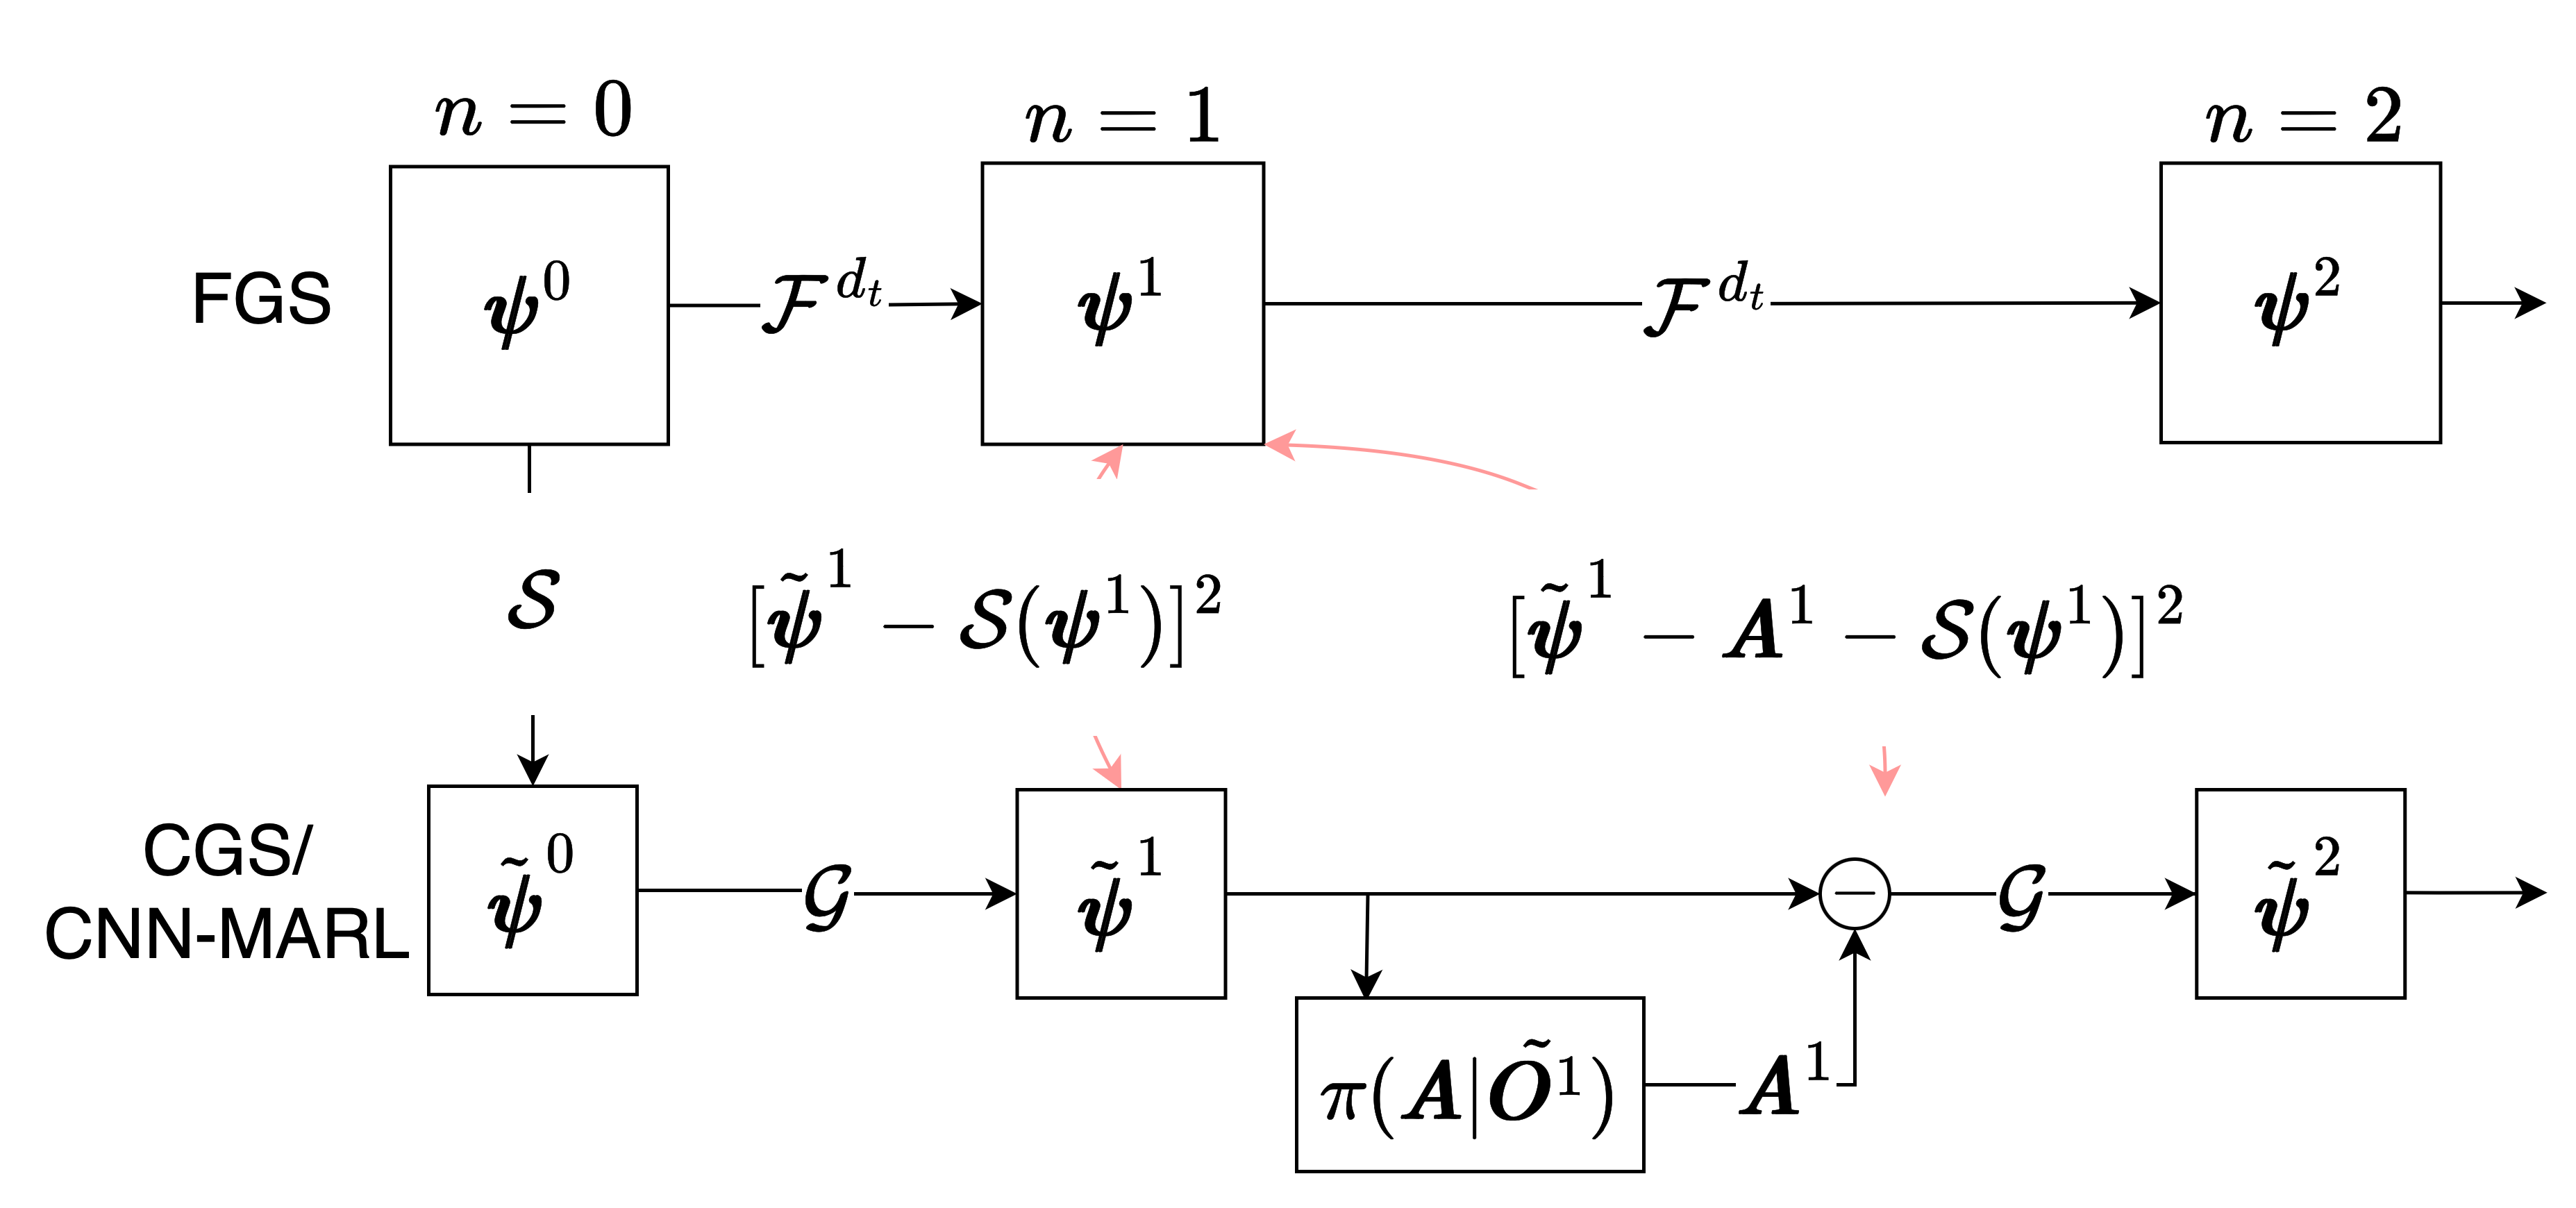
\includegraphics[width=\columnwidth]{illustrations/SMARL_final.drawio.png}}
\caption{Illustration of the training environment with the agents embedded in the CGS. The reward measures how much the action taken improves the CGS.}
\label{fig:environment}
\end{center}
\vskip -0.2in
\end{figure}

The environment of our RL framework is summarized in \cref{fig:environment}. We define the state at step $n$ of the RL environment as the tuple $\boldsymbol{S}^n := (\boldsymbol{\psi}^n, \tilde{ \boldsymbol{\psi}^n})$. This state is only partially observable as the policy is acting only in the CGS. The observation is defined as the coarse representation of the discretized solution function and the parameters $\boldsymbol{O}^n:=(\tilde{ \boldsymbol{\psi}^n}, \tilde C^n) \in \mathcal O$. Our goal is to train a policy $\pi$ that makes the dynamics of the CGS to be close to the dynamics of  the FGS. To achieve this goal, the action ${\boldsymbol{ A}^n} \in \mathcal A :=  \mathbb{R}^{k \times N_x \times N_y }$ at step $n$ of the environment is a collection of forcing terms for each discretization point of the CGS. In case the policy is later used to complement the CGS simulation the update function in \cref{eq:cg_dyn} changes to 
\begin{equation}
   \tilde{\boldsymbol{\psi}}^{n+1}=\mathcal G(\tilde{\boldsymbol{ \psi}}^n - {\boldsymbol{ A}^n}, \tilde C^n). 
\end{equation}
To encourage learning a policy that represents the non-resolved spatio-temporal scales, the reward is based on the difference between the CGS and FGS at time step $n$. In more detail, we define a local reward $\boldsymbol{R}^n \in \mathbb R^{\tilde N_x\times \tilde N_y}$ inspired by the reward proposed for image reconstruction in \cite{cv_pixel_rl}:
\begin{equation}
R_{ij}^n = \frac{1}{k} \sum_{w=1}^k \left([\tilde{\boldsymbol{ \psi}^n} - \mathcal S(\boldsymbol{\psi}^n)]^2 - [\tilde{\boldsymbol{ \psi}^{n}} - {\boldsymbol{ A}^n} - \mathcal S(\boldsymbol{\psi}^n)]^2 \right)_{wij}
\end{equation}
Here, the square $[\cdot]^2$ is computed per matrix entry. We note that the reward function therefore returns a matrix that gives a scalar reward for each discretization point of the CGS.
If the action $\boldsymbol{A}^n$ is bringing the discretized solution function of the CGS $\tilde{\boldsymbol{ \psi}^n}$ closer to the subsampled discretized solution function of the FGS $\mathcal{S}(\boldsymbol{ \psi}^n)$, the reward is positive, and vice versa. In case $\boldsymbol{A}^n$ corresponds to the zero matrix, the reward is the zero matrix as well.\\
During the training process, the objective is to find the optimal policy $\pi^*$ that maximizes the mean expected reward per discretization point given the discount rate $\gamma$ and the observations:
\begin{equation}
\label{eq:pol_old}
\pi^*  =\underset{\pi}{\operatorname{argmax }}\; \mathbb E_{\boldsymbol{\pi}}\left(\sum_{n=0}^{\infty} \gamma^n \bar{r}^{n}\right)
\end{equation}
with the mean expected reward
\begin{equation}
\bar{r}^{n}  =\frac{1}{\tilde N_x\cdot \tilde N_y} \sum_{i,j=1}^{\tilde N_x, \tilde N_y}  R_{ij}^{n}.
\end{equation}

\subsection{Multi-Agent Formulation} 
\label{sec:marl}
The policy $\boldsymbol{\pi}$ predicts a local action $ \boldsymbol{A}^n_{i,j} \in \mathbb R^k$ at each discretization point which implies a very high dimensional  continuous action space. Hence, formulating the closures  with a single agentis very challenging. However, since the rewards are designed to be inherently local, locality can be used as inductive bias and the RL learning framework can be interpreted as a multi-agent problem \cite{cv_pixel_rl}. One agent is placed at each discretization point of the coarse grid with a  corresponding local reward $R_{ij}^n$. We remark  that this approach augments adaptivity as  one can place extra agents at additional, suitably selected, discretization points.\\
Each agent develops its own optimal policy and \cref{eq:pol_old} is replaced by 
\begin{equation} \label{eq:CNN-MARL_objective}
\pi_{ij}^*=\underset{\pi_{ij}}{\operatorname{argmax}} \ \mathbb E_{\pi_{ij}}\left(\sum_{t=0}^{\infty} \gamma^t  R_{ij}^{n}\right),
\end{equation}
Here, we used $\mathcal O (\tilde N_x \tilde N_y)$ agents, which for typically used  grid sizes used in  numerical simulations, it becomes a large number compared to typical MARL problem settings \cite{albrecht2023multi}.\\
We parametrize the local policies using neural networks. However, since training this many individual neural nets can become  computationally expensive, we parametrize all the agents together using  one fully convolutional network (FCN) \cite{fcn}.

\subsection{Parallelizing Local Policies with a FCN}  
All local policies are parametrized using one FCN such that one forward pass through the FCN computes the forward pass for all the agents at once. This approach enforces the aforementioned locality and the receptive field of the FCN corresponds to the spatial neighborhood that an agent at a given discretization point can observe.\\
We define the collection of policies in the FCN as 
\begin{equation}
    \Pi^{FCN}: \mathcal O  \rightarrow \mathcal{A}
\end{equation} 
In further discussions, we will refer to $\Pi^{FCN}$ as the \textit{global policy}. The policy $\pi_{ij}$ of the agent at point $(i,j)$ is subsequently implicitly defined through the global policy as 
\begin{equation}
    \pi_{ij}( O_{ij}) := \left [ \Pi^{FCN} (\boldsymbol O)\right ]_{:ij}.
\end{equation}
Here, $ O_{ij}$ contains only a part of the input contained in $\boldsymbol O$ \footnote{The exact content of $O_{ij}$ is depending on the receptive field of the FCN}. For consistency, we will refer to $\boldsymbol O_{ij}$ as a \textit{local observation} and $\boldsymbol O$ as the \textit{global observation}. We note that the policies $\pi_{ij}(O_{ij})$ map the observation to a probability distribution at each discretization point (see \cref{sec:nn} for details).

Similar to the global policy, the global value function is parametrized using a FCN as well. It maps the global observation to an expected return $H \in  \mathcal{H
} :=R^{ \tilde N_x \times \tilde N_y}$ at each discretization point
\begin{equation}
\mathcal V^{FCN}: \mathcal O \rightarrow \mathcal{H}.
\end{equation}
Similarly to the local policies, we define the \textit{local value function} related to the agent at point $(i,j)$ as $v_{ ij}( O_{ij}) :=  [ \mathcal V^{FCN}(\boldsymbol O) ]_{ij}.$

\subsection{Algorithmic Details} \label{sec:algorithmic_details}
In order to solve the  optimization problem in \cref{eq:CNN-MARL_objective} with the PPO algorithm \cite{ppo}, we modify the single agent approach.\\
Policy updates are performed by taking gradient steps on
\begin{equation}
\mathbb{E}_{\boldsymbol S, \boldsymbol A \sim \Pi^{FCN}} \left[ \frac{1}{\tilde N_x\cdot \tilde N_y} \sum_{i,j=1}^{\tilde N_x, \tilde N_y} L_{\pi_{ij}}(O_{ij},  \boldsymbol{A}_{ij}) \right]
\end{equation}
with the local version of the PPO objective $L_{\pi_{ij}}( O_{ij},  \boldsymbol{A}_{ij})$. This corresponds to the local objective of the policy of the agent at point $(i,j)$ \cite{ppo}.

The global value function is trained on the MSE loss
\[ L_{\mathcal{V}}(\boldsymbol O^n, \boldsymbol{G}^n) =  ||\mathcal V^{FCN}(\boldsymbol O^n)- \boldsymbol{G}^n||_2^2 \]
where $\boldsymbol{G}^n\in \mathbb R^{\tilde N_x\times \tilde N_y}$ represents the actual global return observed by interaction with the environment and is computed as $\boldsymbol{G}^n=\sum_{i=n}^N \gamma^{i-n} \boldsymbol{R}^i$. Here, $N$ represents the length of the respective trajectory.\\
We have provided an overview of the modified PPO algorithm in \cref{appendix:ppo} together with further details regarding the local version of the PPO objective $L_{\pi_{ij}}( O_{ij},  \boldsymbol{A}_{ij})$. Our implementation of the adapted PPO algorithm is based on the single agent PPO algorithm of the Tianshou framework \cite{tianshou}.

\subsection{Neural Network Architecture}
\label{sec:nn}
\begin{figure}[ht]
\vskip 0.2in
\begin{center}
\centerline{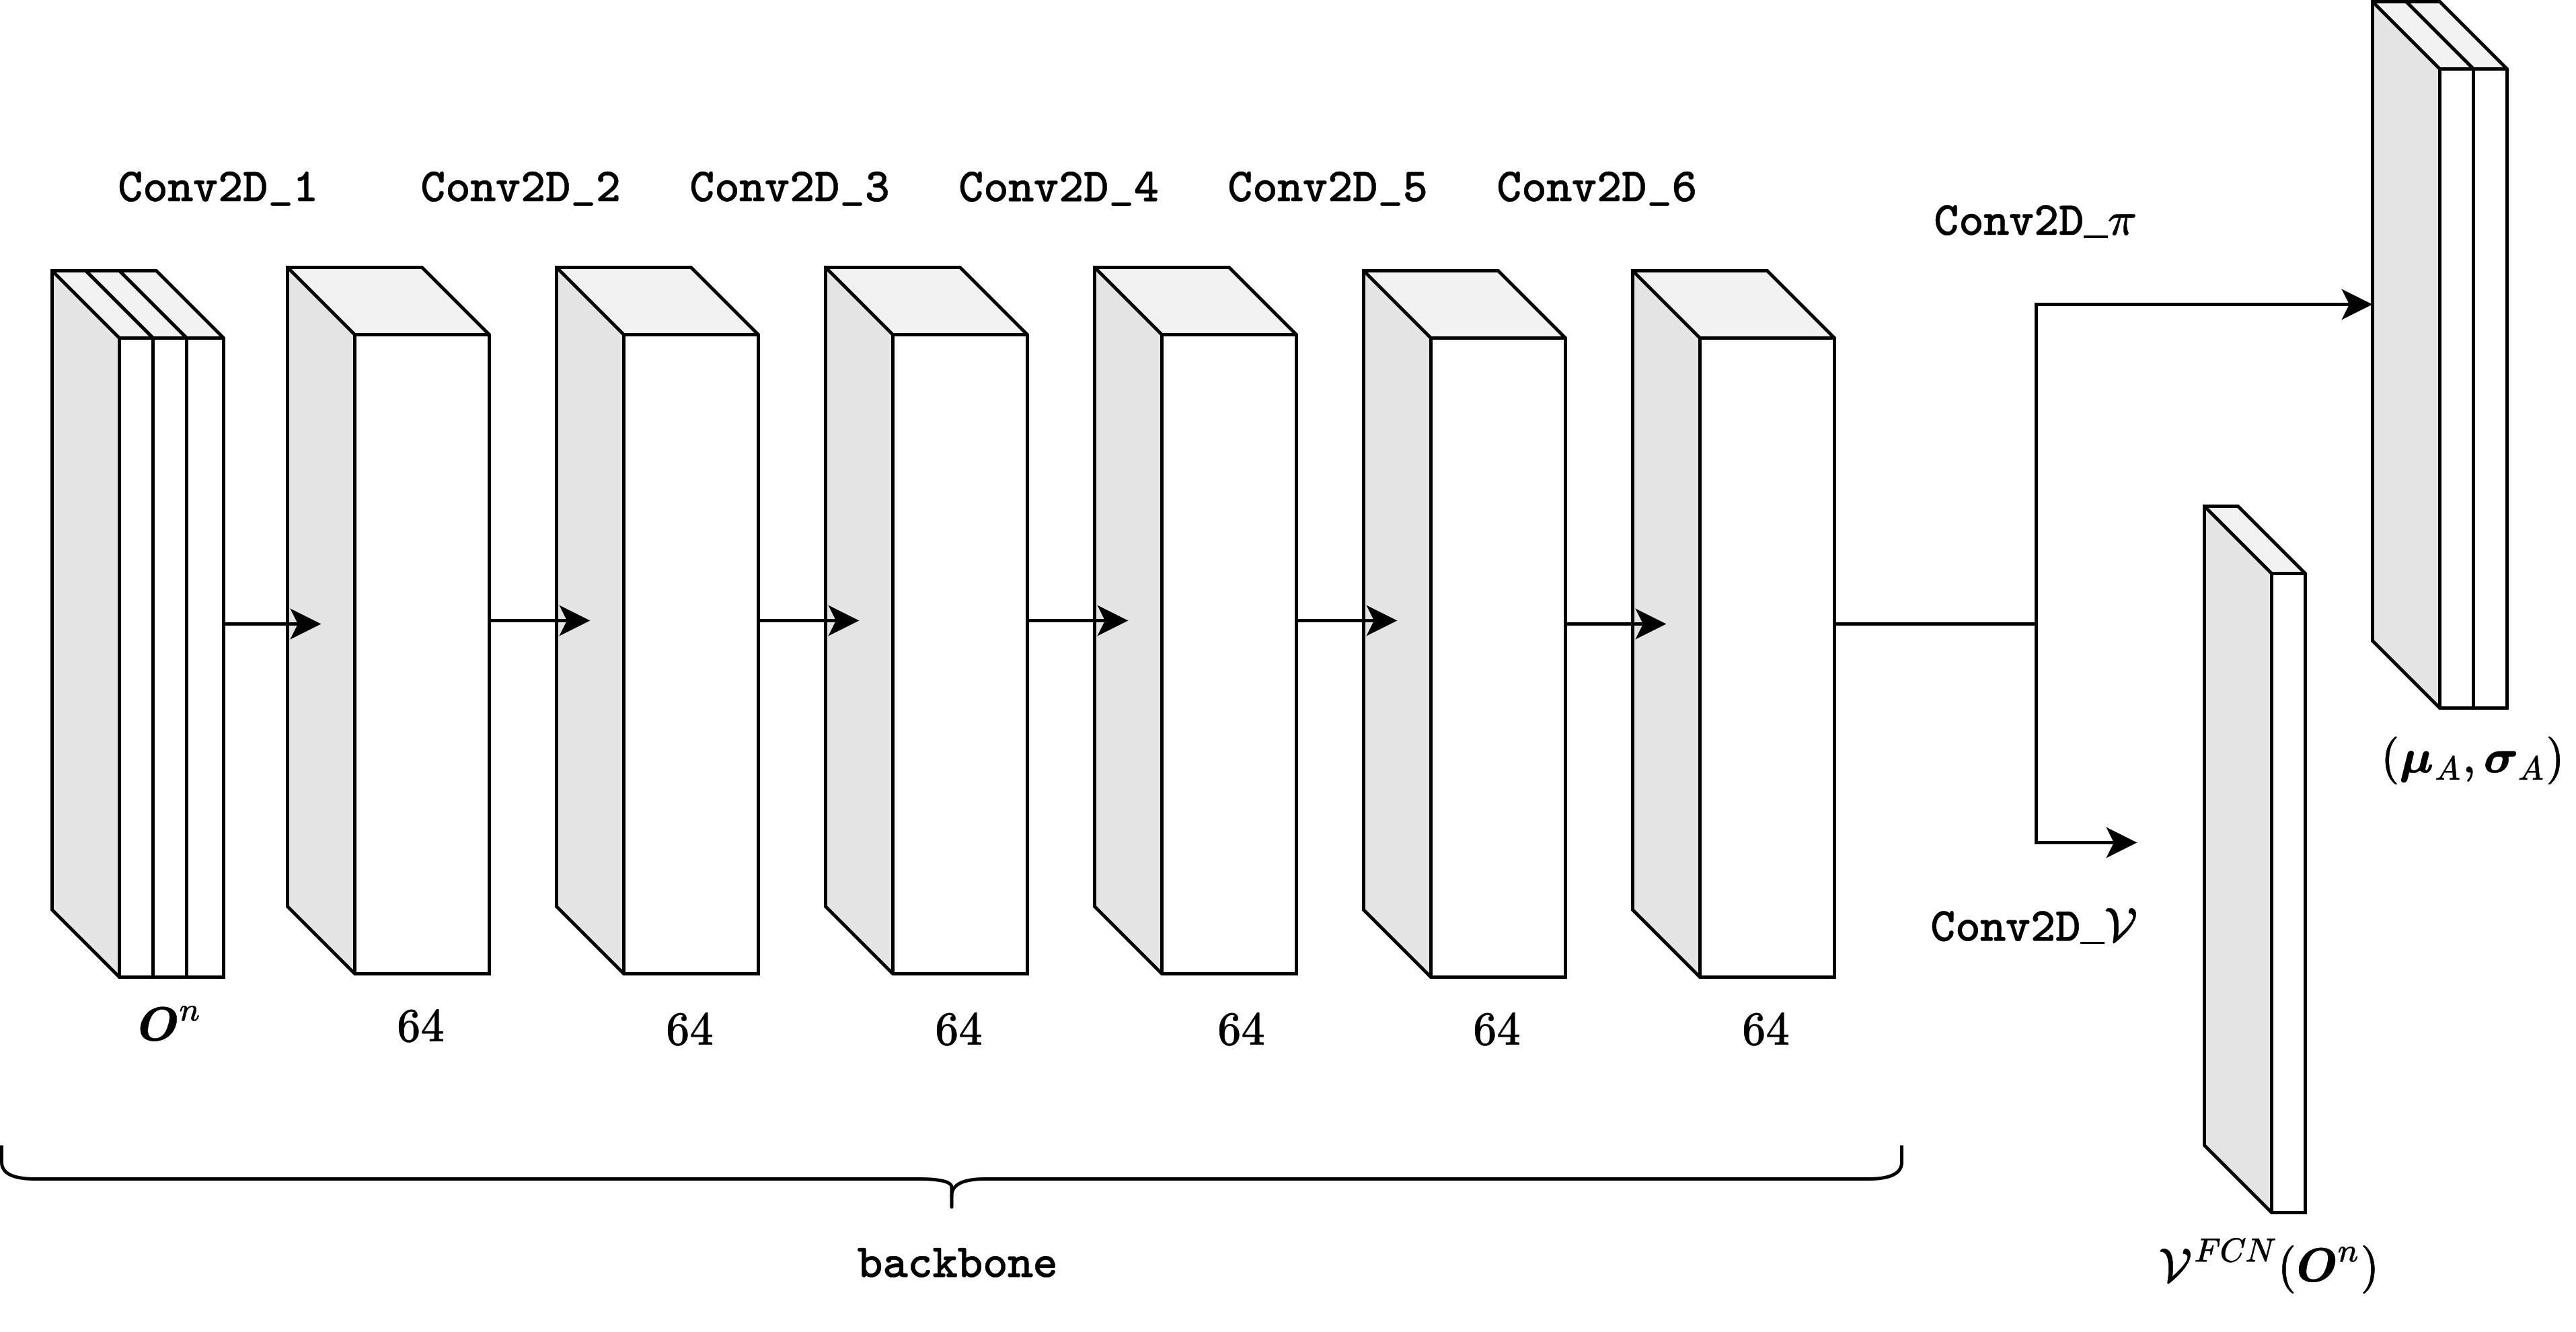
\includegraphics[width=\columnwidth]{illustrations/IRCNN_compr.drawio.png}}
\caption{The IRCNN backbone takes the current global observation and maps it to a feature tensor. This feature tensor is passed into two different convolutional layers that predict the per-discretization point Gaussian parameters and state-values. In the case of a PDE with three spatial dimensions, the architecture would need to be based on three-dimensional convolutional layers instead. }
\label{fig:ircnn}
\end{center}
\vskip -0.2in
\end{figure}
The optimal policy is expected to compensate for errors introduced by the numerical method and its implementation on a  coarse grid. We use the Image Restoration CNN (IRCNN) architecture proposed in \cite{ircnn} as our backbone for the policy- and value-network. In \cref{fig:ircnn} we present an illustration of the architecture and show that the policy- and value network share the same backbone. The policy- and value network only differ by their last convolutional layer, which takes the features extracted by the backbone and maps them either to the parameters $\boldsymbol \mu_A \in \mathcal A$ and $\boldsymbol \sigma_A \in \mathcal A$ or the predicted return value for each agent.  The local policies are assumed to be independent, such that we can write the distribution at a specific discretization point as
\begin{equation}
\pi_{ij}( \boldsymbol{A}_{ij}| O_{ij}) = \mathcal N( \boldsymbol{\mu}_{A,ij},  \boldsymbol{\sigma}_{A,ij}).
\end{equation}
During training, the actions are sampled to allow for exploration, and during inference only the mean is taken as the action of the agent.\\
We note that the padding method used for the FCN can incorporate boundary conditions into the architecture. For instance, in the case of periodic boundary conditions, we propose to use circular padding that involves wrapping around values from one end of the input tensor to the other. \\
In the following, we are referring to the proposed MARL framework using a FCN for both the policy and the value function as CNN-based multi-agent reinforcement learning (CNN-MARL).

\subsection{Computational Complexity}
We note that the computational complexity of the CGS w.r.t. the number of discretization points scales with $\mathcal O(\tilde N_x \tilde N_y)$. As one forward pass through the FCN also scales with $\mathcal O(\tilde N_x \tilde N_y)$ the same is true for CNN-MARL. The FGS employs a finer grid, which leads to a computational cost that scales with $\mathcal O(d_t d ^2 \tilde N_x \tilde N_y)$. This indicates a scaling advantage for CNN-MARL compared to a FGS. Based on these considerations and as shown in the next section in the experiments, CNN-MARL is able to compress some of the computations that are performed on the fine grid as it is able to significantly improve the CGS while keeping the execution time below that of the FGS.

\section{Experiments}
\label{sec:exp}
\subsection{Advection Equation}
First we apply CNN-MARL to the 2D advection equation\footnote{The code to reproduce all results in this paper can be found at (URL added upon publication).}:
\begin{equation}
\frac{\partial \psi}{\partial t} + u(x,y)\frac{\partial \psi}{\partial x} + v(x,y)\frac{\partial \psi}{\partial y} = 0,
\end{equation}
where $\psi$ represents a physical concentration that is transported by the velocity field $C=(u, v)$. We employ periodic boundary conditions (PBCs) on the domain \(\Omega = [0, 1] \times [0, 1]\).\\
For the FGS, this domain is discretized using $N_x=N_y=256$ discretization points in each dimension. To guarantee stability, we employ a time step that ensures that the Courant–Friedrichs–Lewy (CFL) \cite{Courant_1928} condition is fulfilled. The spatial derivatives are calculated using central differences and the time stepping uses the fourth-order Runge-Kutta scheme \cite{quarteroni2008numerical}. The FGS is fourth order accurate in time and second order accurate in space.\\
We construct the CGS by employing the subsampling factors $d=4$ and $d_t=4$.  Spatial derivatives in the CGS use an  upwind scheme and time stepping is performed with the forward Euler method, resulting in first order accuracy in both space and time. All simulation parameters for CGS and FGS are summarized in \cref{tab:advection_params}.

\subsubsection{Initial Conditions}
In order to prevent overfitting and promote  generalization, we design the initializations of $\psi, u$ and $v$ to be different for each episode while still fulfilling the PBCs and guaranteeing the incompressibility of the velocity field. 
The velocity fields are sampled from a distribution $\mathcal D^{Vortex}_{Train}$ by taking a linear combination of Taylor-Greene vortices and an additional random translational field. Further details are provided in \cref{sec:train_vortices}. For visualization purposes, the concentration of a new episode is set to a random sample from the MNIST dataset \cite{mnist} that is scaled to values in the range $[0, 1]$. In order to increase the diversity of the initializations, we augment the data by performing random rotations of $\pm 90 ^{\circ}$ in the image loading pipeline.
\begin{figure*} 
\centering
    \subfigure{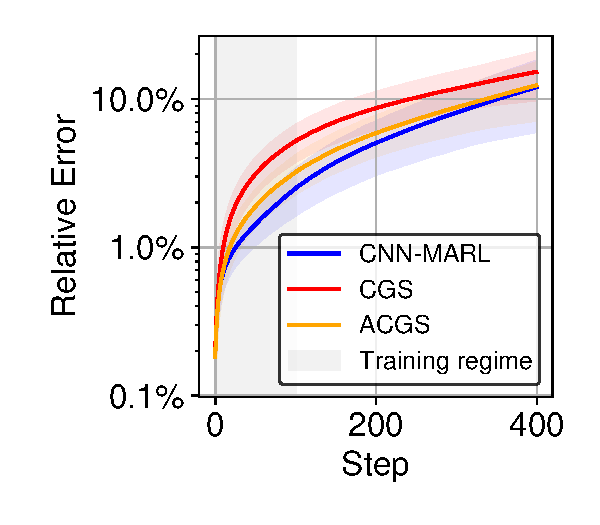
\includegraphics[width=0.24\textwidth]{figures/advection/relative_MAE_evol_400steps_100sims.pdf}}
    \subfigure{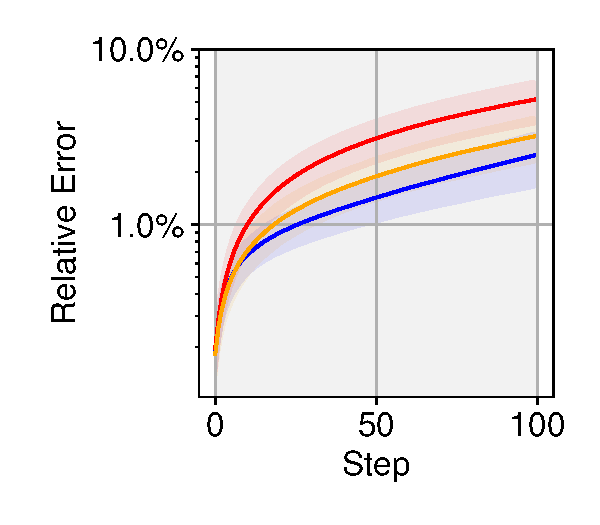
\includegraphics[width=0.24\textwidth]{figures/advection/relative_MAE_evol_100steps_100sims.pdf}}
    \subfigure{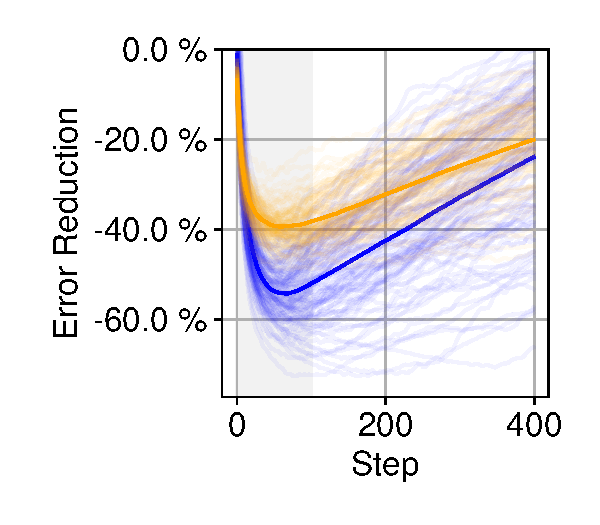
\includegraphics[width=0.24\textwidth]{figures/advection/outperformance_evol_400steps_100sims.pdf}}
    \subfigure{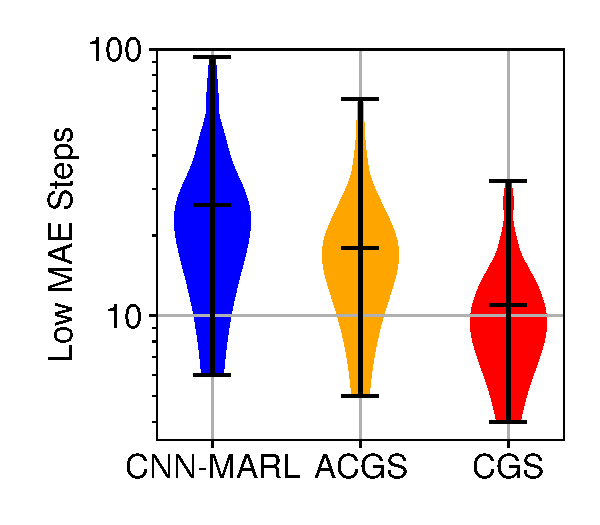
\includegraphics[width=0.24\textwidth]{figures/advection/low_MAE_0.01_violin400steps_100sims.pdf}}
    \caption{Results of CNN-MARL applied to the advection equation. The relative MAEs are computed over 100 simulations with respect to (w.r.t.) the FGS. The shaded regions correspond to the respective standard deviations. The violin plot on the right shows the number of simulation steps until the relative MAE w.r.t. the FGS reaches the threshold of $1\%$.}
    \label{fig:advection_rollout}
\end{figure*}

\subsubsection{Training}
\label{Sec:train}
We train the framework for a total of 2000 epochs and collect 1000 transitions in each epoch. More details regarding the training process as well as the training time  are provided in \cref{sec:training_hyperparams}.\\
We note that the amount and length of episodes varies during the training process:
The episodes are truncated based on the relative Mean Absolute Error ($\text{MAE}$) defined as $\text{MAE}(  \psi^n, \tilde{ \psi^n}) = \frac{1}{\tilde N_x\cdot \tilde N_y}\sum_{i,j} |\psi^n_{ij}- \tilde{\psi}^n_{ij}| / \psi_{max}$
between the CGS and FGS concentrations. Here, $\psi_{max}$ is the maximum observable value of the concentration $\psi$. If this error exceeds the threshold of $1.5 \%$, the episode is truncated. This ensures that during training, the CGS and FGS stay close to each other so that the reward signal is meaningful. As the agents become better during the training process, the mean episode length increases as the two simulations stay closer to each other for longer.\\
We designed this adaptive training procedure in order to obtain stable simulations. 

\subsubsection{Accurate Coarse Grid Simulation}
We also introduce the \textit{'accurate coarse grid simulation'} (ACGS) in order to further compare the effecst of numerics and grid size in CGS and FGS. ACGS operates on the coarse grid, just like the CGS, with a higher order numerical scheme, than the CGS, so that it has the same order of accuracy as the FGS.

\subsubsection{In- and Out-of-Distribution MAE}
\begin{figure}[ht]
\vskip 0.2in
\begin{center}
\centerline{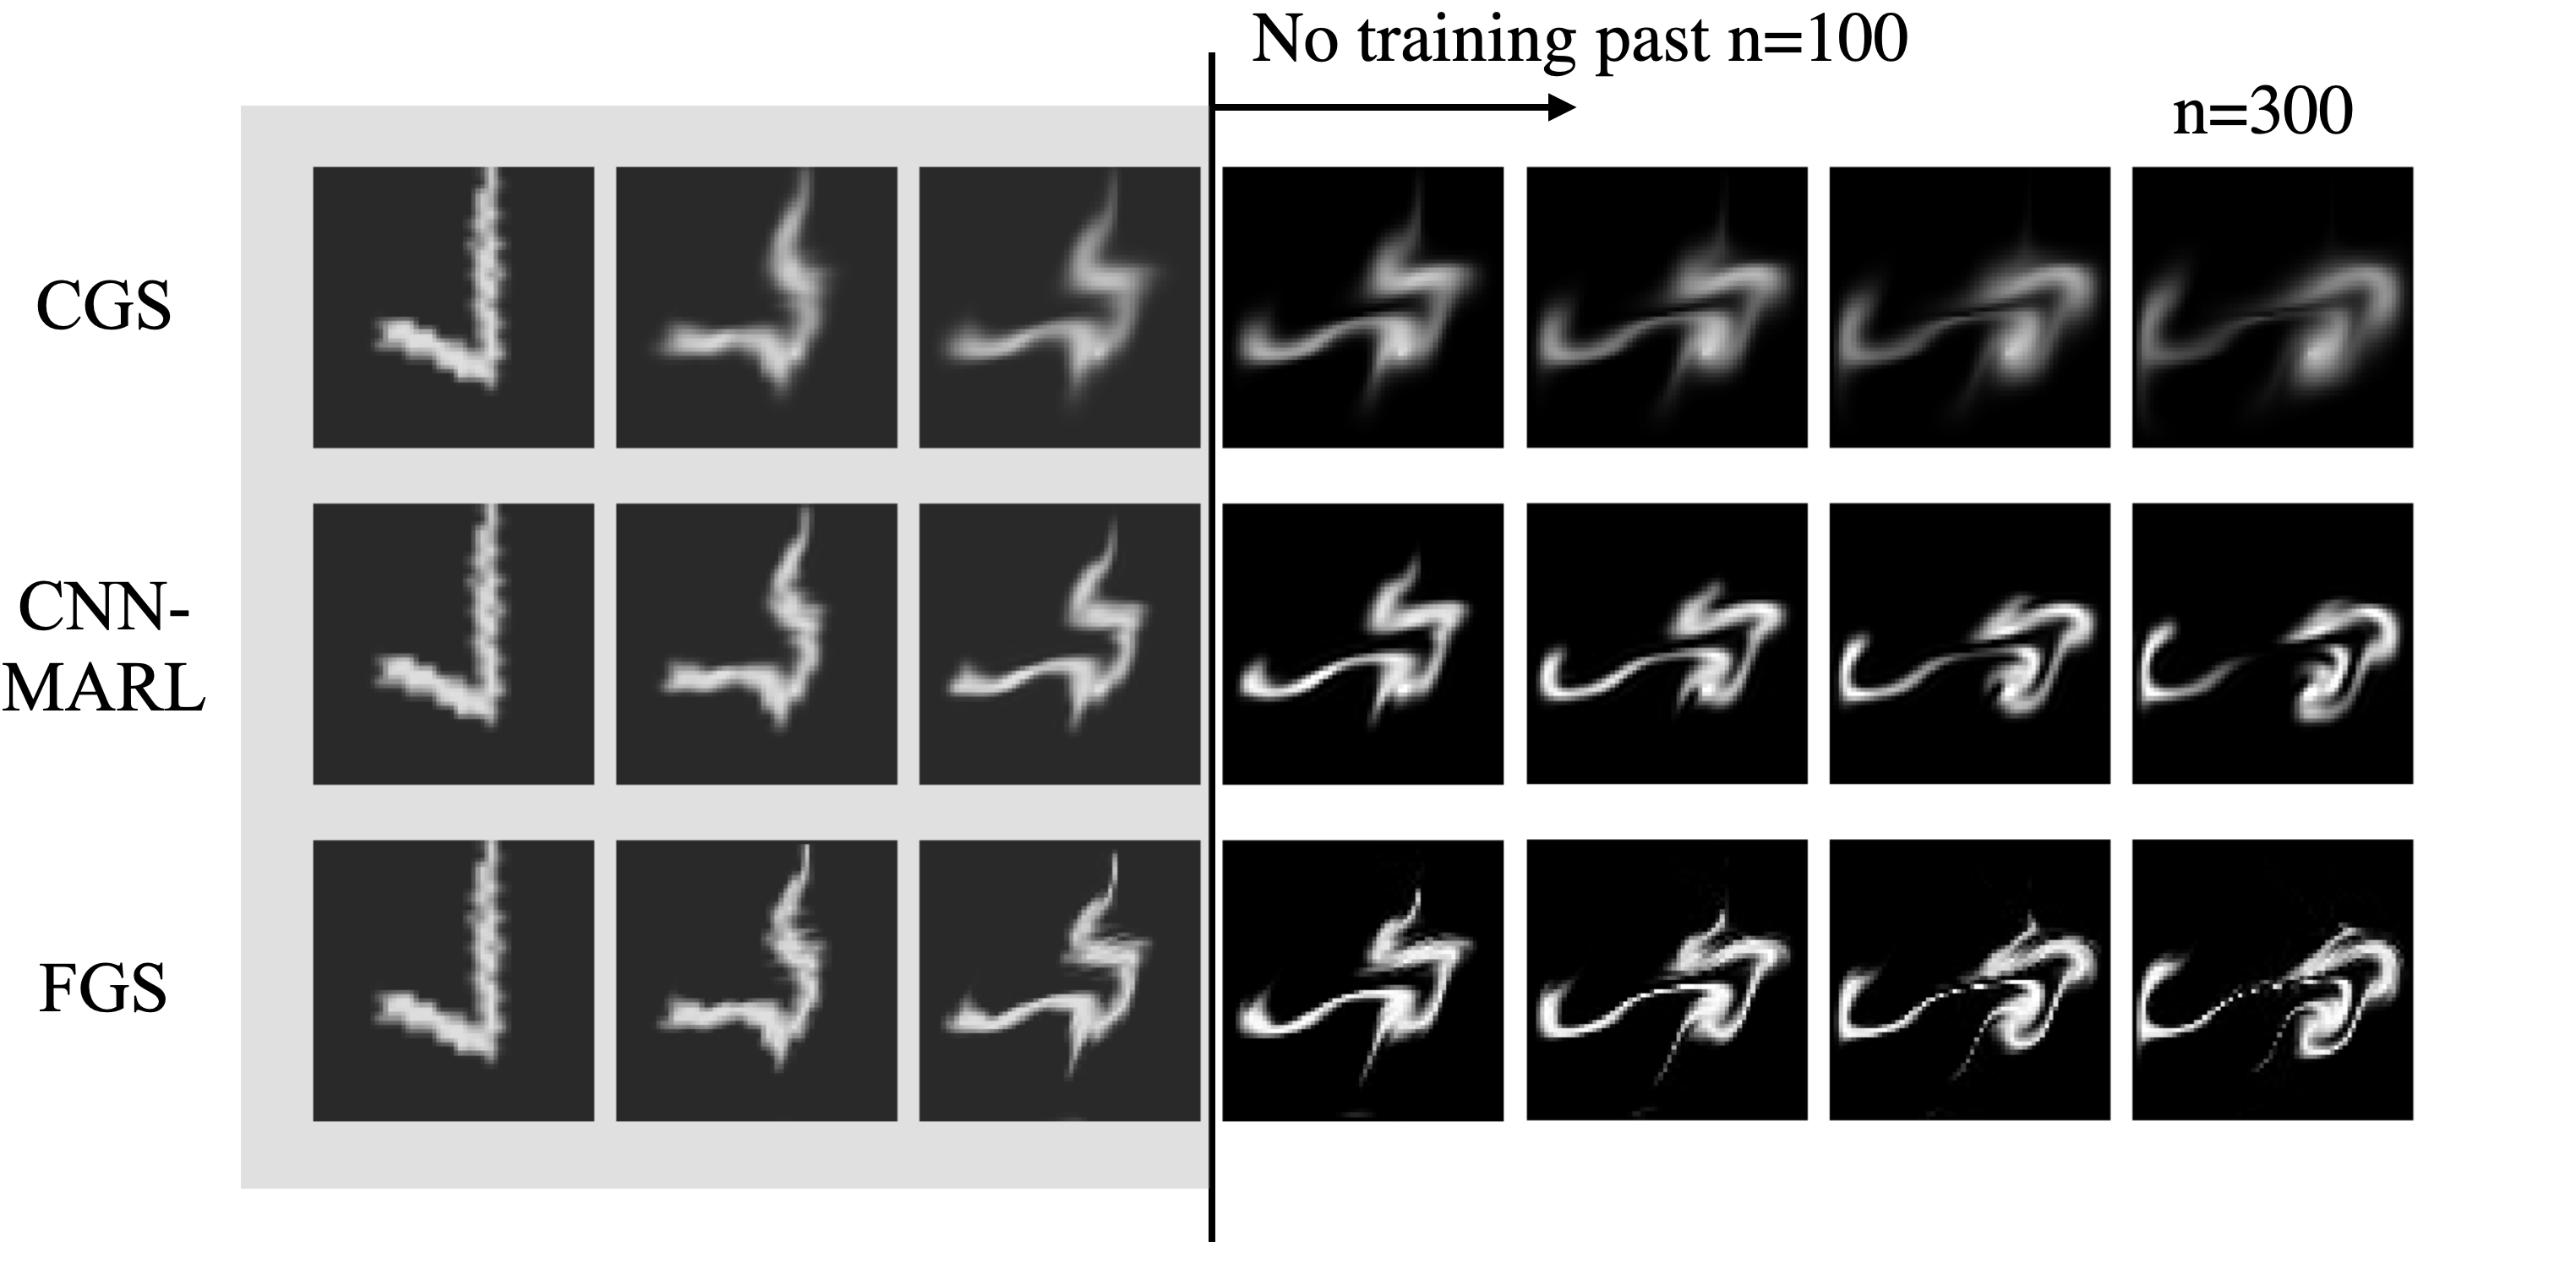
\includegraphics[width=\columnwidth]{illustrations/advection/mnist_train_illustration.png}}
\caption{Example run comparing CGS, CNN-MARL and FGS with the same ICs. The concentration is sampled from the test set and the velocity components are randomly sampled from $\mathcal D^{Vortex}_{Train}$. Note that the agents of the CNN-MARL method have only been trained up to $n=100$. However, they qualitatively improve the CGS simulation past that point.}
\label{fig:advection_example}
\end{center}
\vskip -0.2in
\end{figure}
We develop  metrics for CNN-MARL by running 100 simulations of 50 time steps each with different ICs. For the in-distribution case, the concentrations are sampled from the MNIST test set and the velocity fields are sampled from $\mathcal D^{Vortex}_{Train}$. To quantify the performance on out-of-distribution ICs, we also run evaluations on simulations using the Fashion-MNIST dataset (F-MNIST) \cite{fashionmnist} and a new distribution, $\mathcal D^{Vortex}_{Test}$, for the velocity fields. The latter is defined in \cref{sec:test_vortices}. The resulting error metrics of CGS, ACGS and CNN-MARL w.r.t. the FGS are collected in \cref{tab:50_step_mae_advection}. A qualitative example of the CGS, FGS and the CNN-MARL method after training is presented in \cref{fig:advection_example}. The example shows that CNN-MARL is able to compensate for the dissipation  that is introduced by the first order scheme and coarse grid in the CGS.
\begin{figure*}
\centering
    \subfigure{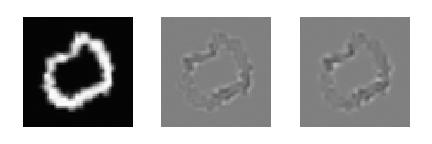
\includegraphics[width=0.65\textwidth]{figures/advection/actions/action_imgs.jpg}}
    \subfigure{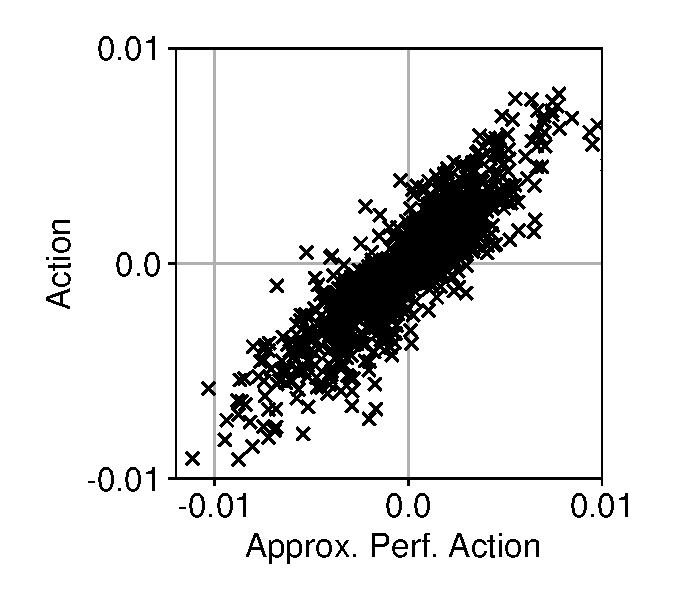
\includegraphics[width=0.24\textwidth]{figures/advection/actions/action_cluster.pdf}}
    \caption{Visual comparison of the input concentration $\tilde{\boldsymbol \psi}^n$, taken actions $\boldsymbol A^n$ and the corresponding numerical approximation of the optimal action from left to right. The figure on the right-hand side qualitatively shows the linear relation between approximated optimal actions and taken actions.}
    \label{fig:action_interpretation}
\end{figure*}

\begin{table}[!ht]
\caption{Relative MAE at time step 50 averaged over 100 simulations with different ICs to both the velocity and concentration. All relative MAE values are averaged over the complete domain and reported in percent.}
\label{tab:50_step_mae_advection}
\vskip 0.15in
\centering
\scriptsize 
\begin{tabular}{@{}l|cccr@{}}
\toprule
Velocity & \multicolumn{2}{c}{$\mathcal D^{Vortex}_{Train}$} & \multicolumn{2}{c}{$\mathcal D^{Vortex}_{Test}$} \\
Concentr. & MNIST & F-MNIST & MNIST & F-MNIST \\
\hline 
CGS & $3.13 \pm 0.80$ & $3.23 \pm 0.92$ & $3.82 \pm 0.78$ & $3.12 \pm 0.73$ \\ 
ACGS & $1.90 \pm 0.51$ & $2.27 \pm 0.64$ & $2.28 \pm 0.47$ & $2.23 \pm 0.50$\\
CNN-MARL & $\textbf{1.46} \pm 0.33$ & $\textbf{2.12} \pm 0.57$  & $\textbf{1.58} \pm 0.37$ & $\textbf{2.04} \pm 0.56$ \\  \bottomrule
\multicolumn{5}{c}{Relative Improvements w.r.t. CGS} \\
 \bottomrule
ACGS &  -39\% &  -30\% &  -40\% &  -31\%\\
 CNN-MARL & \textbf{-53\%} & \textbf{-34\%} & \textbf{-58\%} & \textbf{-36\%} \\ 
 \bottomrule
\end{tabular}
\end{table}
CNN-MARL reduces the relative MAE of the CGS after 50 steps by $30\%$ or more in both in- and out-of-distribution cases. This shows that the agents have learned a meaningful correction for the truncation errors of the numerical schemes in the coarser grid. 

CNN-MARL also outperforms the ACGS w.r.t. the MAE metric which indicates that the learned corrections  emulate a higher-order scheme. This indicates that the proposed methodology is  able to emulate the unresolved dynamics and is a suitable option for complementing existing numerical schemes.

We note the strong performance of our framework w.r.t. the out-of-distribution examples. For both unseen and out-of-distribution ICs as well as parameters, the framework was able to outperform CGS and ACGS. In our opinion, this indicates that we have discovered an actual model of the forcing terms that goes beyond the training scenarios. 

\subsubsection{Evolution of Numerical Error}
The results in the previous sections are mostly focused on the difference between the methods after a rollout of 50 time steps. To analyze how the methods compare over the course of a longer rollout, we analyze the relative MAE at each successive step of a simulation with MNIST and $\mathcal D^{Vortex}_{Train}$ as distributions for the ICs. The results are shown in \cref{fig:advection_rollout}. 

The plots of the evolution of the relative error show that CNN-MARL is able to improve the CGS for the entire range of a 400-step rollout, although it has only been trained for 100 steps. This implies that the agents are seeing distributions of the concentration that have never been encountered during training and are able to generalize to these scenarios. When measuring the duration of simulations for which the relative error stays below $1\%$, we observe that the CNN-MARL method outperforms both ACGS and CGS, indicating that the method is able to produce simulations with higher long term stability than CGS and ACGS. We attribute this to our adaptive scheme for episode truncation during training as introduced in \cref{Sec:train} and note that the increased stability can be observed well beyond the training regime.

\subsubsection{Interpretation of Actions}
\label{sec:int}
We are able to derive the optimal update rule for the advection CGS that negates the errors introduced by the numerical scheme (see \cref{sec:proof_optimal_action} for the derivation):
\begin{equation}
\tilde{\boldsymbol\psi}^{n+1} = \mathcal G (\tilde{\boldsymbol\psi}^{n} - \widetilde{\Delta t} \tilde{\boldsymbol\epsilon}^{n-1}, \tilde C^n),
\end{equation}
Here, $ \tilde{\boldsymbol\epsilon}^{n-1} \in \mathbb R^{\tilde N_x \times \tilde N_y}$ is the truncation error of the previous step. However, note that there exists no closed-form solution to calculate the truncation error $\tilde{\boldsymbol\epsilon}^{n-1}$ if only the state of the simulation is given.\\
We therefore employ a numerically approximate for the truncation errors for further analysis:
\begin{equation}
\small{\tilde \epsilon^{n} = \frac{\widetilde{\Delta t}}{2} \tilde \psi_{tt}^n + |\tilde u^n| \frac{\widetilde{\Delta x}}{2}\tilde \psi_{xx}^n + |\tilde v^n| \frac{\widetilde{\Delta y}}{2}\tilde \psi_{yy}^n + \mathcal O(\widetilde{\Delta t}^2, \widetilde{\Delta x}^2, \widetilde{\Delta y}^2)}
\end{equation}
Here $\tilde \psi_{xx}^n$,$\tilde \psi_{yy}^n$ and $\tilde \psi_{tt}^n$ are second derivatives of $\psi$ that are numerically estimated using second-order central differences.\\
We compare the obtained optimal update rule for the CGS with the predicted mean action $\boldsymbol \mu_A$ of the policy and thus the learned actions. \cref{fig:action_interpretation} visualizes an example, which indicates that there is a strong linear relationship between the predicted mean action and the respective numerical estimate of the optimal action. \\
In order to further quantify the similarity between the numerical estimates of $- \widetilde{\Delta t} \tilde{\epsilon}^{n-1}_{i,j}$ and the taken action, we compute the Pearson product-moment correlation coefficient for 100 samples. The results are presented in \cref{tab:action_correlation} and show that the learned actions as well as the optimal action of the CGS are highly correlated for all different combinations of seen and unseen ICs and parameters. 
\begin{table}[!ht]
\caption{Mean and standard deviation of Pearson product-moment correlation coefficients between $\boldsymbol \mu_A^n$ and numerically approximated $- \widetilde{\Delta t} \tilde{\boldsymbol\epsilon}^{n-1}$ for 100 samples for different combinations of velocity fields and initializations of the concentration.}
\vskip 0.15in
\centering
\begin{tabular}{@{}l|cr@{}}
\toprule
 & MNIST & F-MNIST  \\
\hline 
$\mathcal D^{Vortex}_{Train}$ & $0.82 \pm 0.05$ & $0.70 \pm 0.08$  \\ 
$\mathcal D^{Vortex}_{Test}$ & $0.82 \pm 0.03$ & $0.72 \pm 0.08$ \\ \bottomrule
\end{tabular}
\label{tab:action_correlation}
\end{table}

\begin{figure*}
\centering
    \subfigure{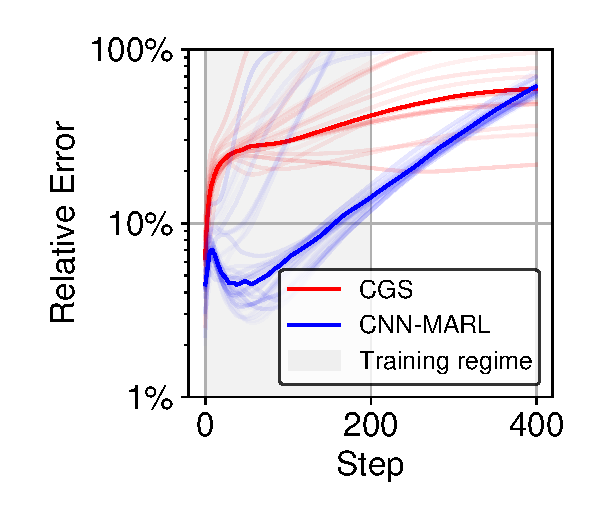
\includegraphics[width=0.24\textwidth]{figures/burgers/relative_MAE_evol_400steps.pdf}}
    \subfigure{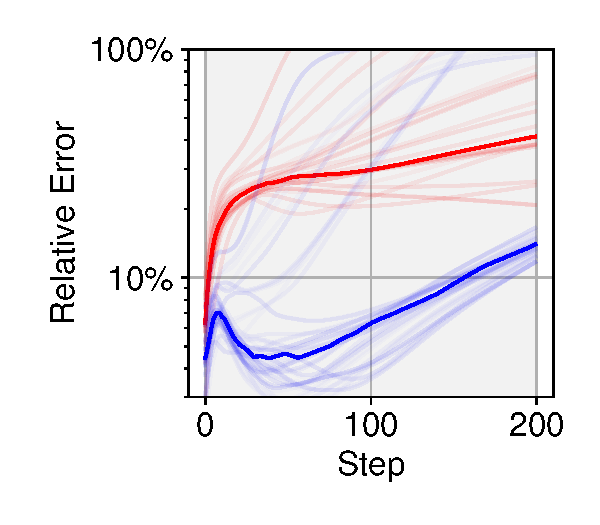
\includegraphics[width=0.24\textwidth]{figures/burgers/relative_MAE_evol_200steps.pdf}}
    \subfigure{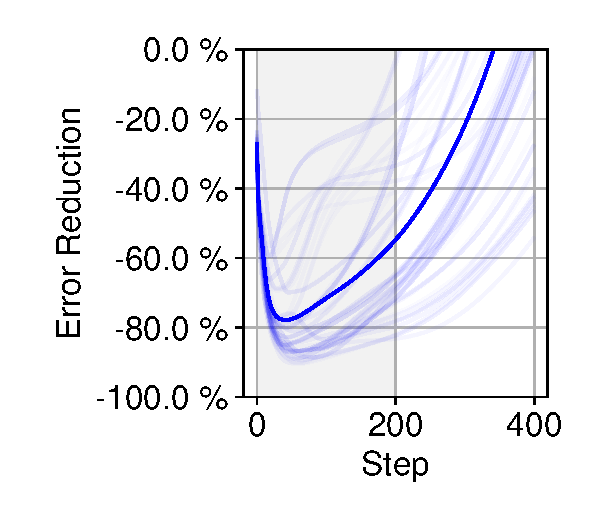
\includegraphics[width=0.24\textwidth]{figures/burgers/improvement_rel_MAE_evol_200steps.pdf}}
    \subfigure{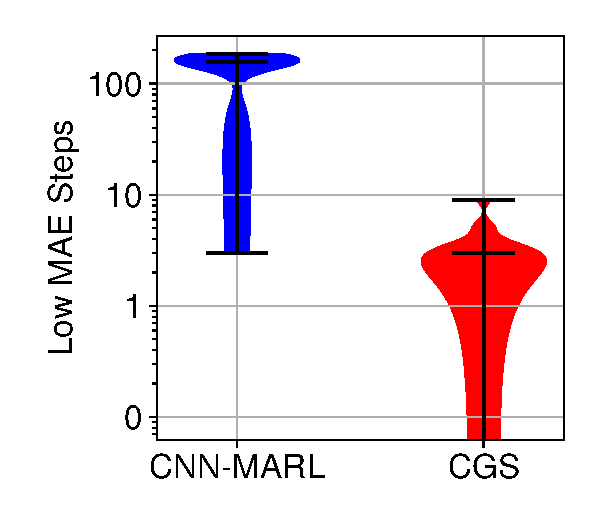
\includegraphics[width=0.24\textwidth]{figures/burgers/low_MAE_0.1_violin400steps_100sims.pdf}}
    \caption{Results of CNN-MARL applied to the Burgers' equation. The relative MAEs are computed over 100 simulations with respect to the FGS. The shaded regions correspond to the respective standard deviations. The violin plot on the right shows the number of simulation steps until the relative MAE w.r.t. the FGS reaches the threshold of $10\%$.}
    \label{fig:burgers_errors}
\end{figure*}

 Additionally, we note that the truncation error contains a second-order temporal derivative. At first glance, it might seem surprising that the model would be able to predict this temporal derivative as the agents can only observe the current time step. However, the observation contains both the PDE solution, i.e. the concentration for the present examples, as well as the parameters of the PDE, i.e. the velocity fields. Thus, both the concentration and velocity field are passed into the FCN and due to the velocity fields enough information is present to infer this temporal derivative.

\subsection{Burgers' Equation}
As a second example, we apply our framework to the 2D viscous Burgers' equation:
\begin{equation}
\frac{\partial \boldsymbol{\psi}}{\partial t} + (\boldsymbol{\psi} \cdot \nabla) \boldsymbol{\psi} - \nu \nabla^2 \boldsymbol{\psi} = 0.
\end{equation}
Here, $\boldsymbol{\psi} := (u, v)$ consists of both velocity components and the PDE has the single input parameter $C=\nu$. As for the advection equation, we assume  periodic boundary conditions on the domain \(\Omega = [0, 1] \times [0, 1]\). 
In comparison to the advection example, we are now dealing with two solution variables and thus $k=2$.\\
For the FGS, the aforementioned domain is discretized using $N_x=N_y=150$ discretization points in each dimension. Moreover, we again choose $\Delta t$ to fulfill the CFL condition for stability (see \cref{tab:burgers_params}). The spatial derivatives are calculated using the upwind scheme and the forward Euler method is used for the time stepping \cite{quarteroni2008numerical}.\\
We construct the CGS by employing the subsampling factors $d=5$ and $d_t=10$. For the Burgers experiment, we apply a mean filter $K$ with kernel size $d\times d$ before the actual subsampling operation. The mean filter is used to eliminate higher frequencies in the fine grid state variables, which would lead to accumulating high errors. The CGS employs the same numerical schemes as the FGS here. This leads to first order accuracy in both space and time. All the simulation parameters for CGS and FGS are collected in \cref{tab:burgers_params}. \\
In this example, where FGS and CGS are using the same numerical scheme, the CNN-MARL framework has to focus solely on negating the effects of the coarser discretization. 

For training and evaluation, we generate random, incompressible velocity fields as ICs (see \cref{sec:train_vortices} for details) and set the viscosity $\nu$ to $0.003$. We observed that the training of the predictions actions can be improved by multiplying the predicted forcing terms with $\widetilde{\Delta t}$. This is consistent with our previous analysis in \cref{sec:int} as the optimal action is also multiplied but this factor. Again, we train the model for 2000 epochs with 1000 transitions each. The maximum episode length during training is set to $200$ steps and, again, we truncate the episodes adaptively, when the relative error exceeds $20 \%$. Further details on training CNN-MARL for the Burgers' equation can be found in \cref{sec:training_hyperparams}. Visualization of the results can be found in \cref{sec:adres} and the resulting relative errors w.r.t. the FGS are shown in \cref{fig:burgers_errors}. The CNN-MARL method again improves the CGS significantly, also past the point of the 200 steps seen during training. Specifically, in the range of step $0$ to step $100$ in which the velocity field changes fastest, we see a significant error reductions up to $-80\%$. When analyzing the duration for which the episodes stay under the relative error of $10\%$, we observe that the mean number of steps is improved by two order of magnitude, indicating that the method is able to improve the long term accuracy of the CGS.  

\section{Conclusion}
We propose a novel methodology (CNN-MARL), for the automated discovery of closure models of coarse grained discretizations of  time-dependent PDEs. We show that CNN-MARL develops a  policy that compensates for numerical errors in a CGS of the 2D advection and Burgers' equation. More importantly we find that, after training, the learned closure model can be used for predictions in extrapolative test cases. In turn, the agent actions are interpretable and highly correlated with the error terms of the numerical scheme.\\
CNN-MARL utilizes a multi-agent formulation with a FCN for both the policy and the value network. This enables the incorporation of  both local and global rewards without necessitating individual neural networks for each agent. This setup allows to efficiently train a large number of agents without the need for decoupled subproblems. Moreover, the framework trains on rollouts without needing to backpropagate through the numerical solver itself.\\A current drawback is the requirement of a regular grid. The framework would still be applicable to an irregular grid, but information about the geometry would need to be added to the observations. Moreover, for very large systems of interest the numerical schemes used are often multi-grid and the 
RL framework should reflect this. For such cases, we suggest defining separate rewards for each of the grids employed by the numerical solver.\\
We believe that the introduced framework holds significant promise for advancing the discovery of closure models in a wide range of systems governed by Partial Differential Equations as well as  other computational methods such as  coarse grained molecular dynamics. 

\newpage
\section*{Broader Impact Statement}
In this paper, we have presented a MARL framework for systematic identification of closure models in coarse-grained PDEs. The anticipated impact pertains primarily to the scientific community, whereas the use in
real-life applications would require additional adjustments and expert input.

% In the unusual situation where you want a paper to appear in the
% references without citing it in the main text, use \nocite
%\nocite{langley00}
%\newpage
\bibliography{references}
\bibliographystyle{icml2023}


%%%%%%%%%%%%%%%%%%%%%%%%%%%%%%%%%%%%%%%%%%%%%%%%%%%%%%%%%%%%%%%%%%%%%%%%%%%%%%%
%%%%%%%%%%%%%%%%%%%%%%%%%%%%%%%%%%%%%%%%%%%%%%%%%%%%%%%%%%%%%%%%%%%%%%%%%%%%%%%
% APPENDIX
%%%%%%%%%%%%%%%%%%%%%%%%%%%%%%%%%%%%%%%%%%%%%%%%%%%%%%%%%%%%%%%%%%%%%%%%%%%%%%%
%%%%%%%%%%%%%%%%%%%%%%%%%%%%%%%%%%%%%%%%%%%%%%%%%%%%%%%%%%%%%%%%%%%%%%%%%%%%%%%
\newpage
\appendix
\onecolumn
\section{Adapted PPO Algorithm} \label{appendix:ppo}
As defined in \cref{sec:algorithmic_details} the loss function for the global value function is 
\[ L_{\mathcal{V}}(\boldsymbol O^n, \boldsymbol{G}^n, \phi) =  ||\mathcal V^{FCN}_{\phi}(\boldsymbol O^n)- \boldsymbol{G}^n||_2^2. \]
We note that this notation contains the parameters $\phi$, which parameterize the underlying neural network.

The objective for the global policy is defined as
\[L_{\Pi}(\boldsymbol O^n, \boldsymbol A^n, \theta_k, \theta, \beta) := \frac{1}{\tilde N_x\cdot \tilde N_y} \sum_{i,j=1}^{\tilde N_x, \tilde N_y} L_{\pi_{ij}}({O}^n_{ij}, {A}^n_{ij}, \theta_k, \theta) - \beta H(\pi_{ij,\theta}),\]
where  $H(\pi_{ij,\theta})$ is the entropy of the local policy and $L_{\pi_{ij}}$ is the standard single-agent PPO-Clip objective
\[ \label{eq:ppo_objective}
L_{\pi_{ij}}(o, a, \theta_k, \theta) = \min \left( \frac{\pi_{ij,\theta}(a|o)}{\pi_{ij,\theta_k}(a|o)} Adv^{\pi_{ij,\theta_k}}(o, a), \text{clip} \left( \frac{\pi_{ij,\theta}(a|o)}{\pi_{ij,\theta_k}(a|o)}, 1 - \epsilon, 1 + \epsilon \right) Adv^{\pi_{ij,\theta_k}}(o, a) \right).
\]
The advantage estimates \( {Adv}^{\pi_{ij,\theta_k}} \) are computed with generalized advantage estimation (GAE) \cite{generalized_advantage_estimation} using the output of the global value network \( \mathcal{V}^{FCN}_{\phi} \).\\

The resulting adapted PPO algorithm is presented in \cref{algo:ppo}. Major differences compared to the original PPO algorithm are vectorized versions of the value network loss and PPO-Clip objective, as well as a summation over all the discretization points of the domain before performing an update step.  

\begin{algorithm}[tb]
   \caption{Adapted PPO Algorithm}
    \label{algo:ppo}
\begin{algorithmic}
   \STATE {\bfseries Input:} Initial policy parameters \( \theta_1 \), initial value function parameters \( \phi_1 \), \\
 clip ratio \( \epsilon\), discount factor \(\gamma\), entropy regularization weight \(\beta\)
   \FOR{\( k = 1, 2, \ldots \)}
   \STATE Collect set of trajectories \( D_k  \) with the  global policy \( \Pi^{FCN}_{\theta_k} \) in the environment
   \STATE \textit{\# Update global policy}
   \STATE Update $\theta$ by performing a SGD step on \( \theta_{k+1} = \arg \max_\theta \frac{1}{\|D_k\|}\sum_{\boldsymbol{O}^n, \boldsymbol G^n \in D_k} L_{\Pi}(\boldsymbol O^n, \boldsymbol A^n, \theta_k, \theta, \beta) \)
   \STATE \textit{\# Update global value network}
    \STATE Compute returns for each transition using \( \boldsymbol{G}^n=\sum_{i=n}^N \gamma^{i-t} \boldsymbol{R}^i \) where $N$ is the length of the respective trajectory
    \STATE Update $\phi$ by performing a SGD step on \( \phi_{k+1} = \arg \min_\phi \frac{1}{\|D_k\|}\sum_{\boldsymbol{O}^n, \boldsymbol G^n \in D_k} L_{\mathcal V}(\boldsymbol{O}^n, \boldsymbol{G}^n, \phi) \)
   \ENDFOR
\end{algorithmic}
\end{algorithm}

\newpage
\section{Additional Results}
\subsection{Advection Equation}
\begin{figure}[ht]
\vskip 0.2in
\begin{center}
\centerline{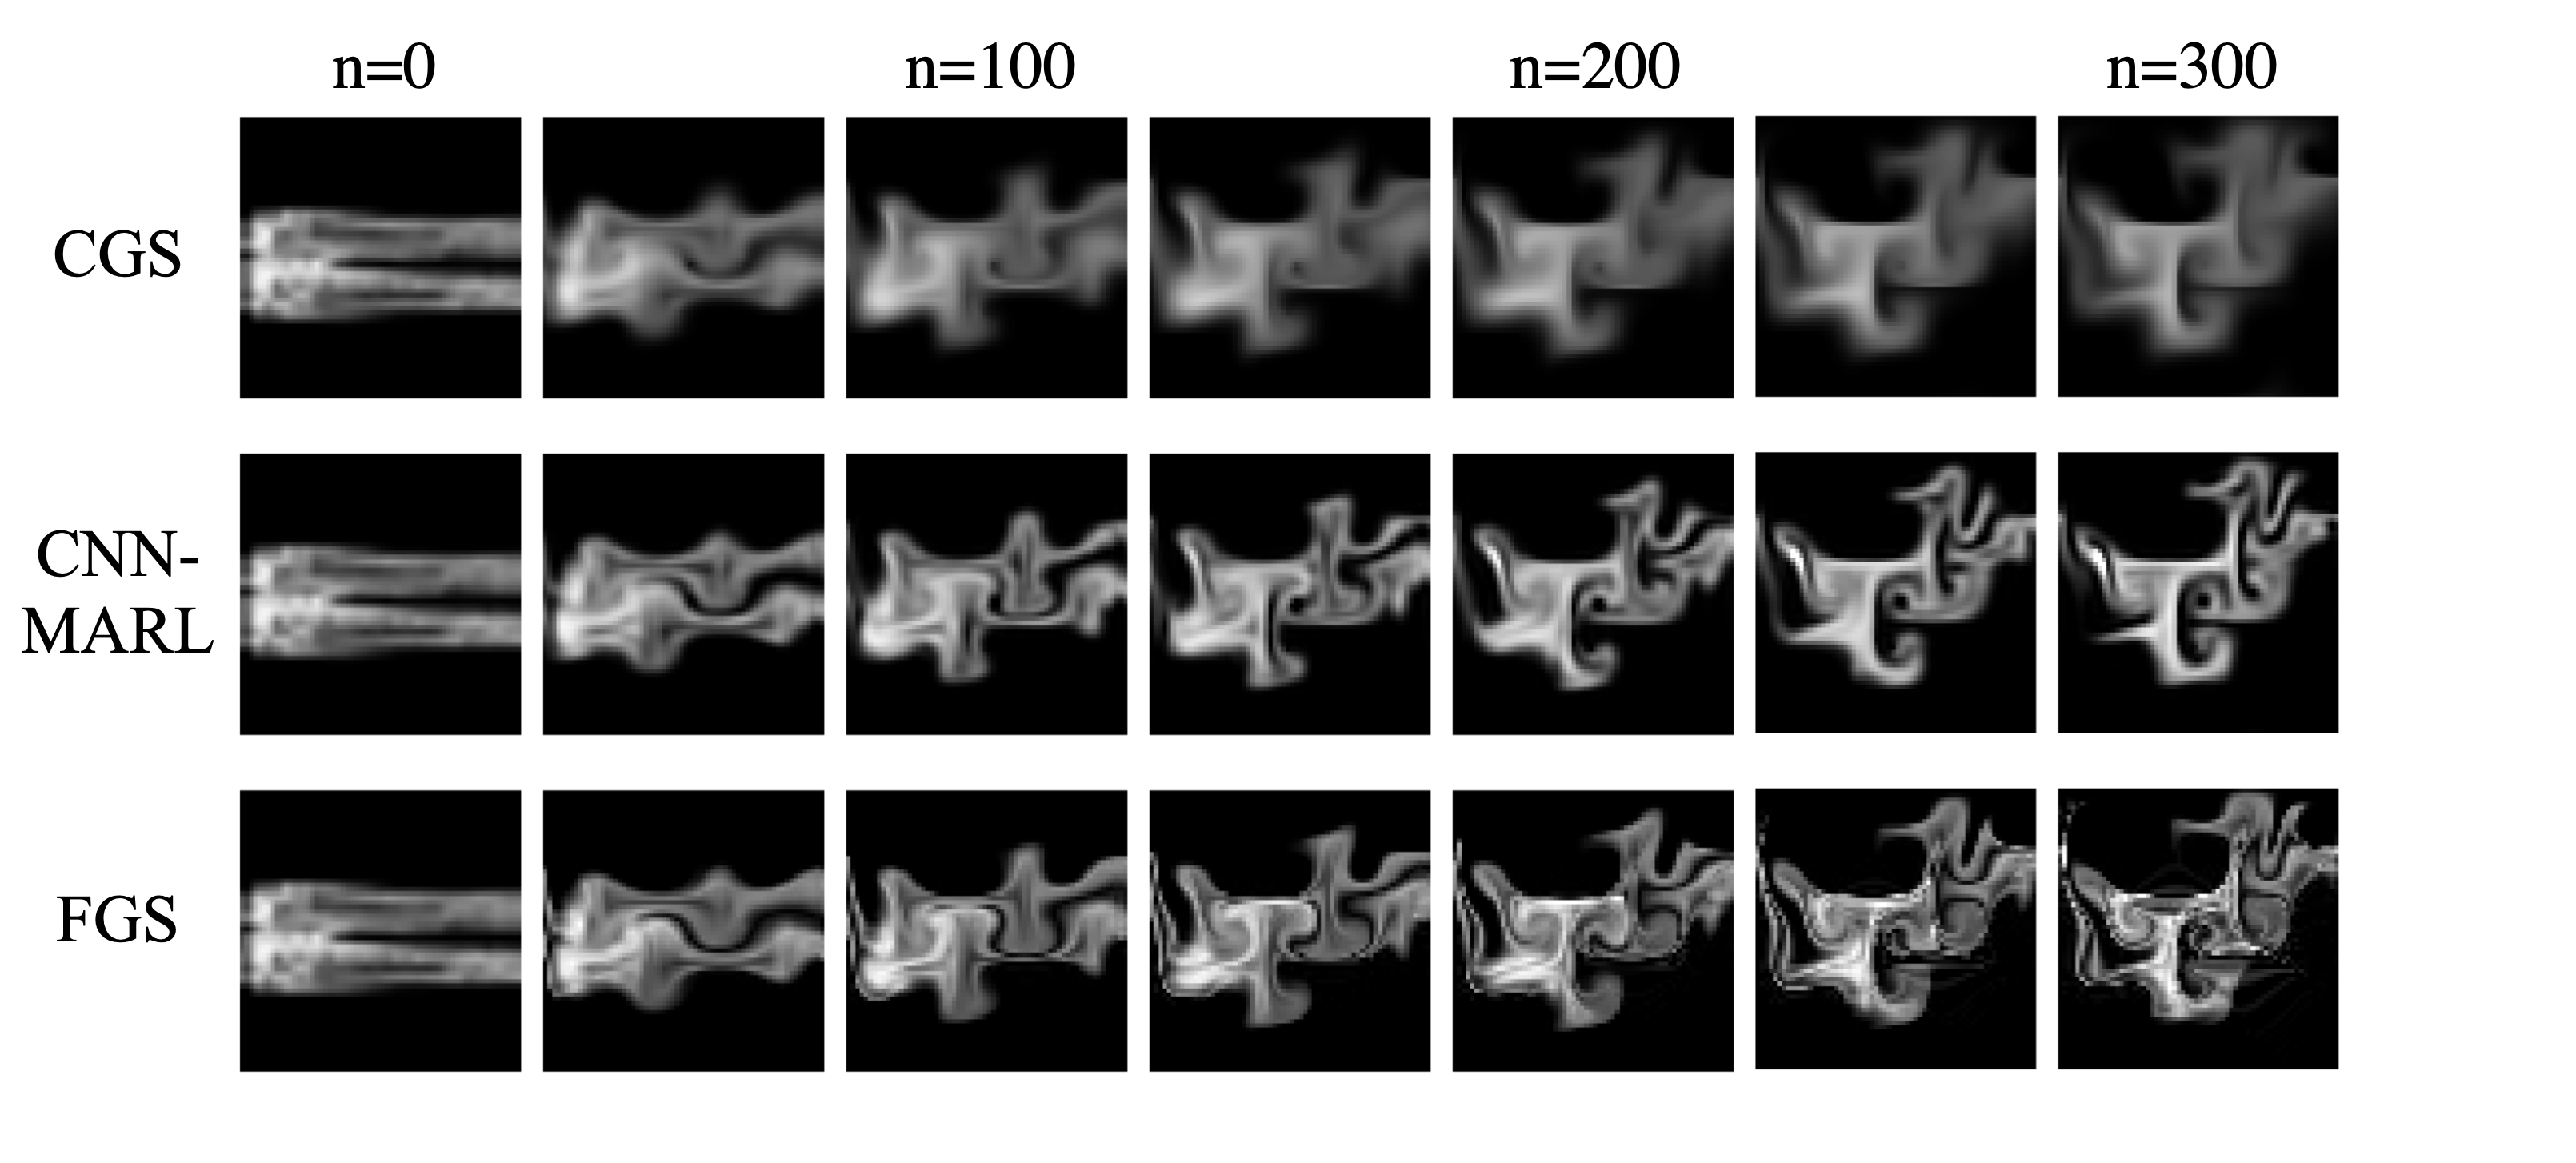
\includegraphics[width=0.75\columnwidth]{illustrations/advection/fashion_train_illustration.png}}
\caption{$\boldsymbol \psi^0$ is sampled from the MNIST test set. The velocity field is sampled from $\mathcal D^{Vortex}_{Test}$ (See \cref{sec:train_vortices}). Here, the IC of the concentration comes from a different distribution than the one used for training.}
\end{center}
\vskip -0.2in
\end{figure}

\begin{figure}[ht]
\vskip 0.2in
\begin{center}
\centerline{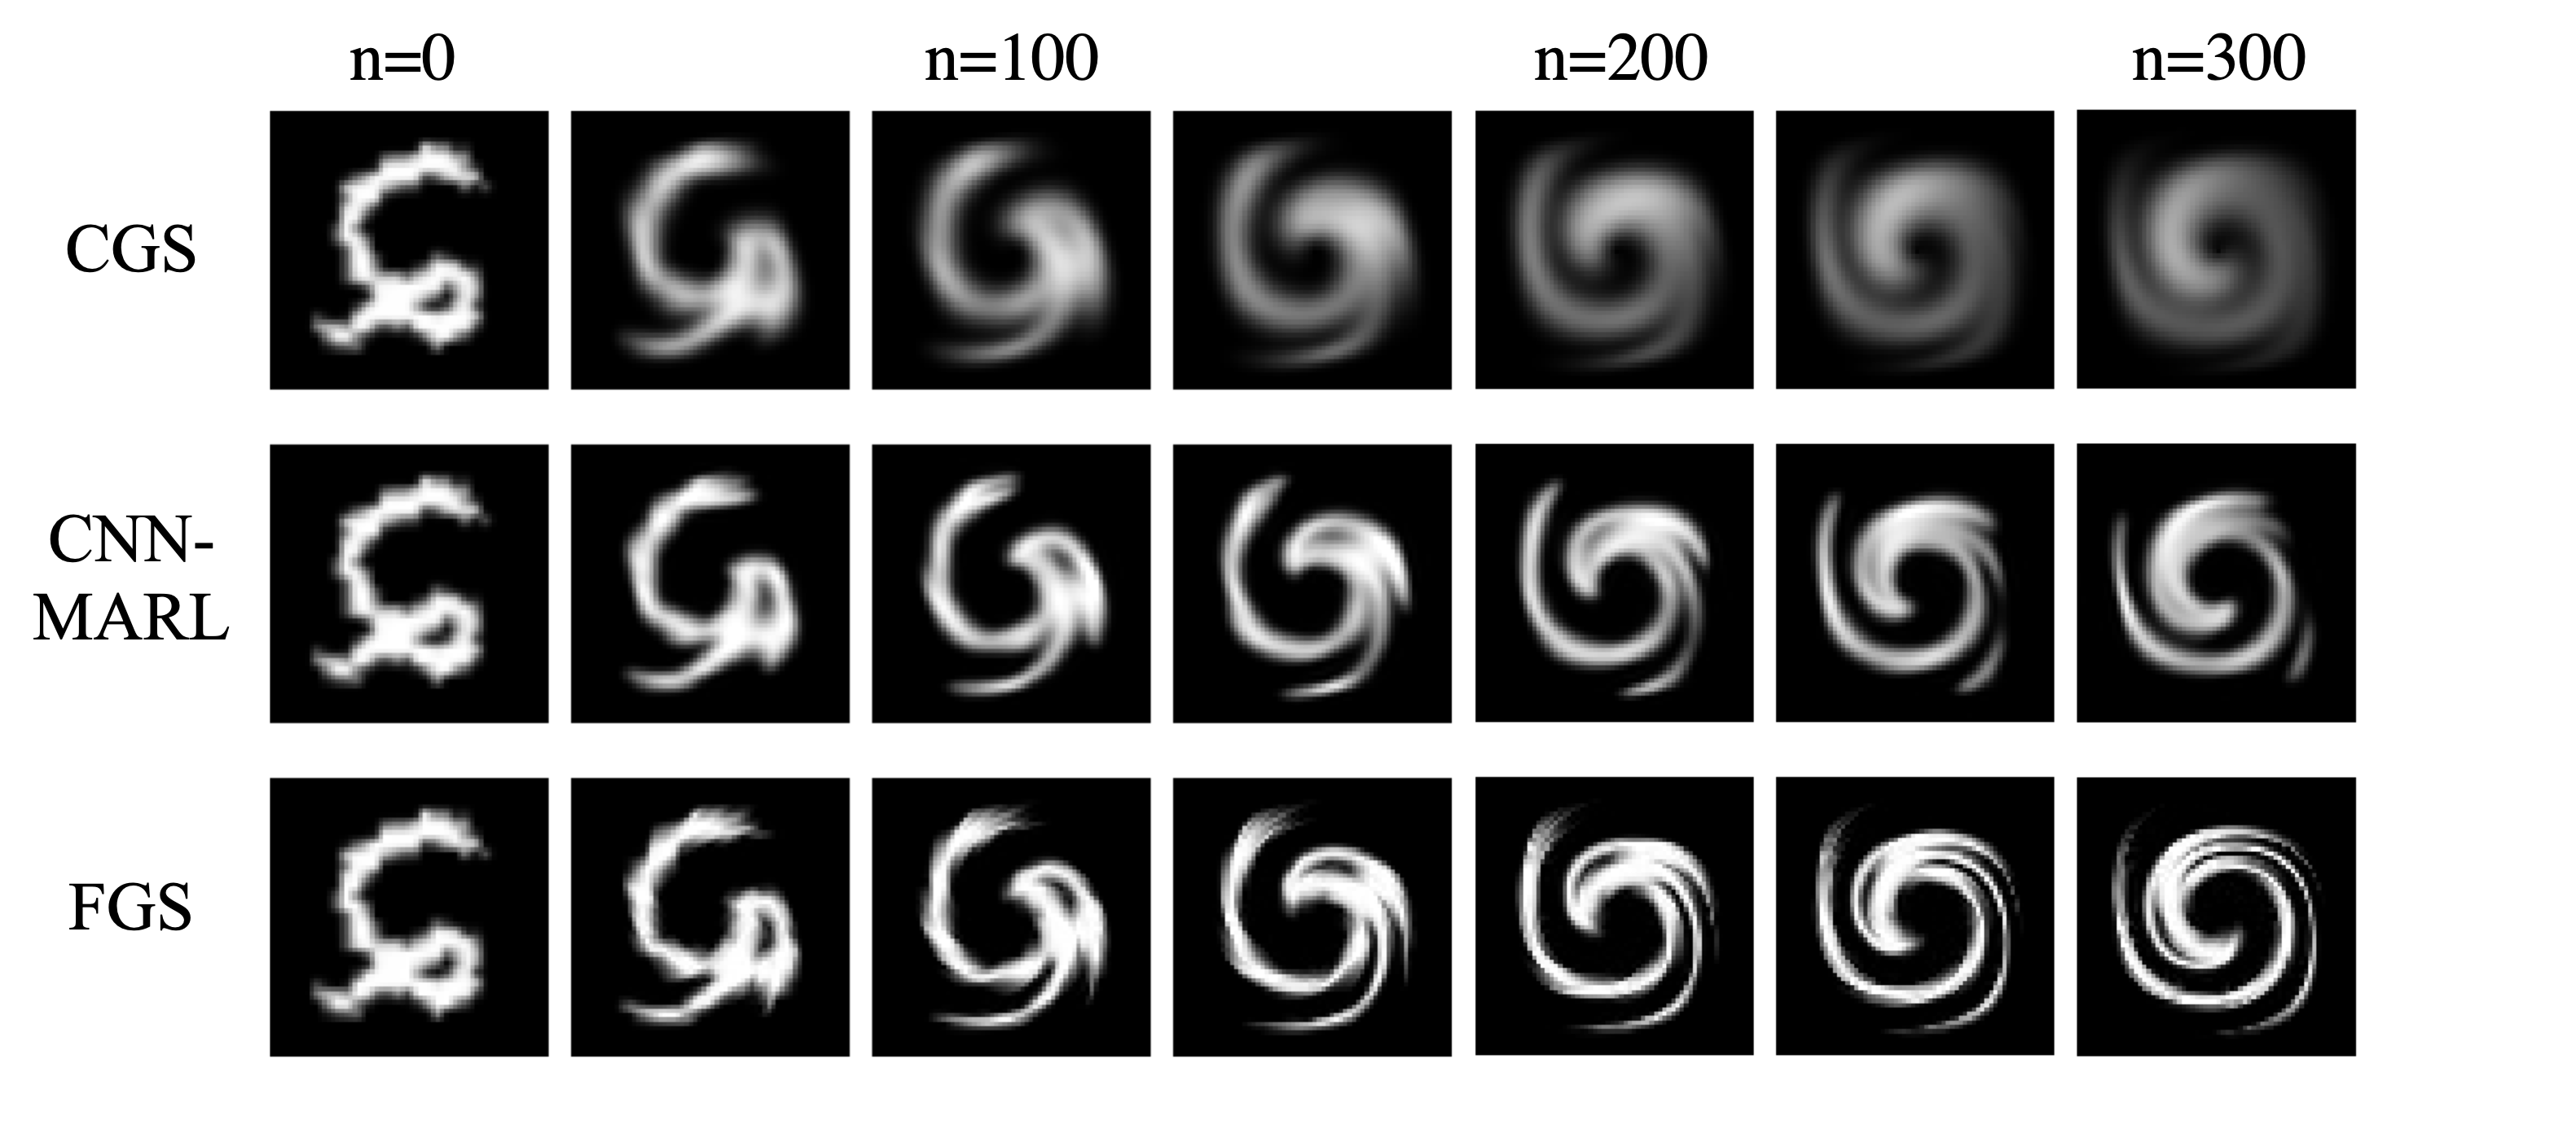
\includegraphics[width=0.75\columnwidth]{illustrations/advection/mnist_vortex_illustration.png}}
\caption{$\boldsymbol \psi^0$ is a sample from the F-MNIST test set. The velocity field is sampled from $\mathcal D^{Vortex}_{Train}$ (See \cref{sec:test_vortices}). Note that the velocity field comes from a different distribution than the one used for training.}
\end{center}
\vskip -0.2in
\end{figure}

\newpage
\subsection{Burgers' Equation}
\label{sec:adres}
\begin{figure}[ht]
\vskip 0.2in
\begin{center}
\centerline{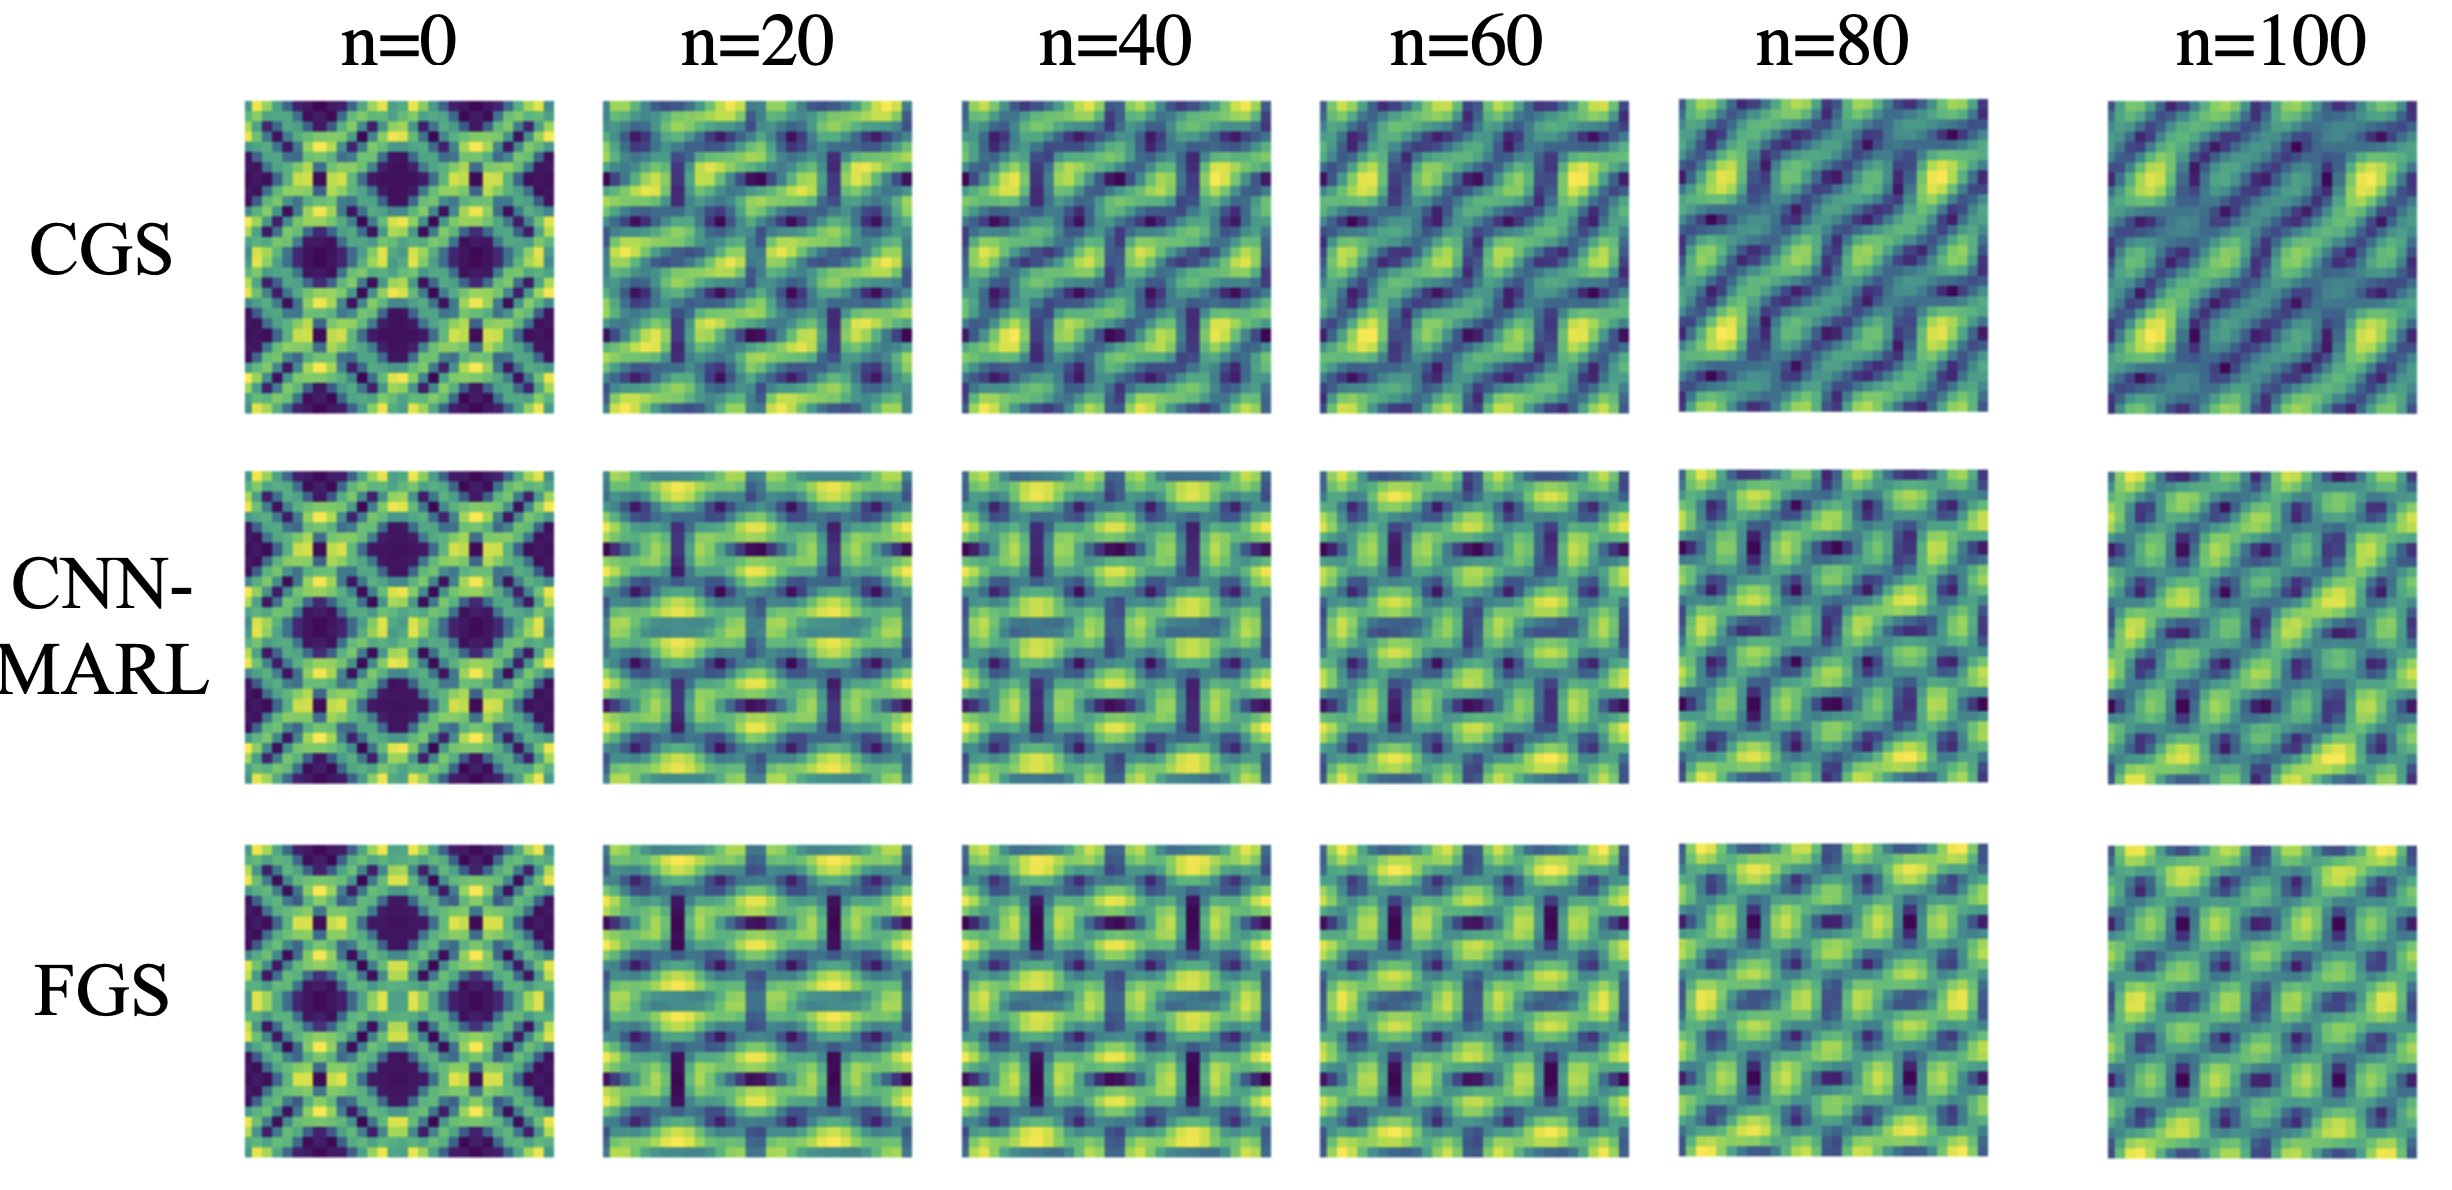
\includegraphics[width=0.75\columnwidth]{illustrations/burgers/burgers_expl1.png}}
\caption{$\boldsymbol \psi^0$ is a sample from $\mathcal D_{Train}^{Vortex}$. We plot the velocity magnitude of every $20$th step of simulation with $100$ coarse time steps. The example shows that CNN-MARL does also qualitatively keep the simulation closer to the FGS. The failure of the CGS to account for the subgrid-scale dynamics leads to diverging trajectories.}
\label{fig:burgers_example}
\end{center}
\vskip -0.2in
\end{figure}

\begin{figure}[ht]
\vskip 0.2in
\begin{center}
\centerline{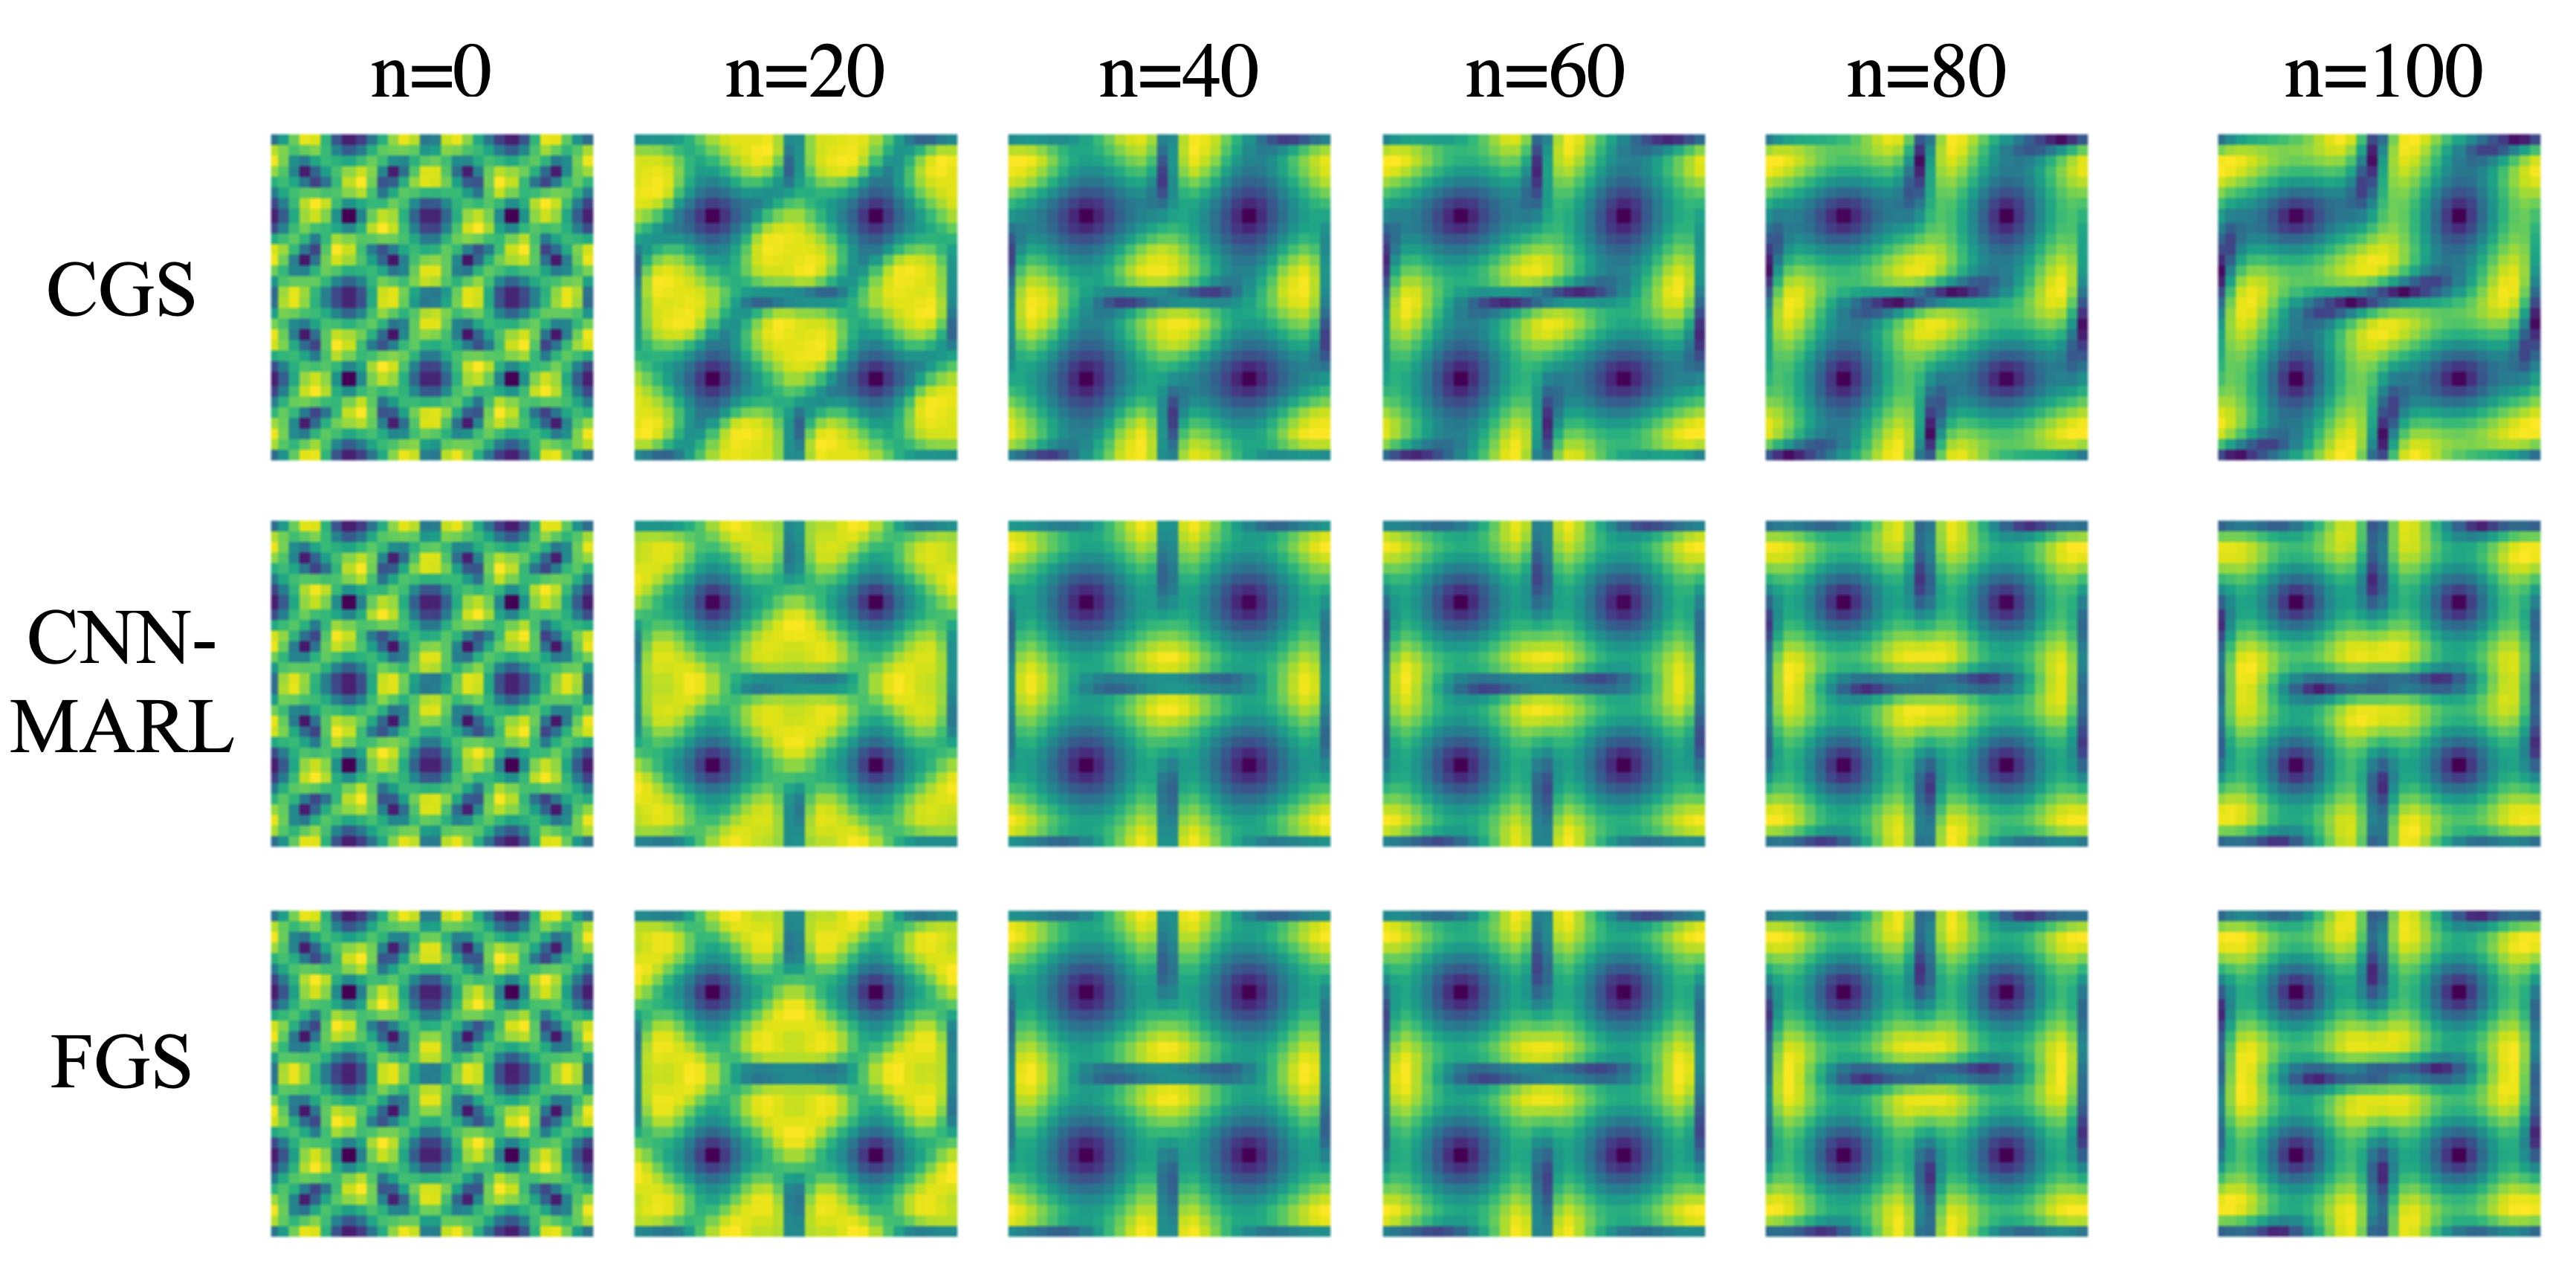
\includegraphics[width=0.75\columnwidth]{illustrations/burgers/burgers_expl2.png}}
\caption{Velocity magnitude plotted for a 100-step roll out. The set-up is the same as in \cref{fig:burgers_example} and the example again shows, that CNN-MARL leads to qualitatively different dynamics during a roll-out that are closer to those of the FGS.}
\end{center}
\vskip -0.2in
\end{figure}

\newpage
\section{Technical Details on Hyperparamters and Training Runs} \label{sec:training_hyperparams}
During training, we use entropy regularization in the PPO objective with a factor of $0.1$ and $0.05$ for the advection and Burgers' equation respectively to encourage exploration. The discount factor is set to $0.95$ and the learning rate to $1\cdot 10^{-5}$. Training is done over 2000 epochs. In each epoch, 1000 transitions are collected. One policy network update is performed after having collected one new episode. We use a batch size of 10 for training. The total number of trainable parameters amounts to $188,163$ and the entire training procedure took about 8 hours for the advection equation on an Nvidia A100 GPU. For the Burgers' equation, training took about $30$ hours on the same hardware. We save the policy every 50 epochs and log the corresponding MAE between CGS and FGS after 50 time steps. For evaluation on the advection equation, we chose the policy from epoch 1500 because it had the lowest logged MAE value. \cref{fig:advection_training_graphs} and \cref{fig:burgers_training_graphs} show the reward curves and evolutions of episode lengths. As expected, the episode length increases as the agents become better at keeping the CGS and FGS close to each other. 

\begin{figure}[h]
    \centering
    \hfill
    \raisebox{-\height}{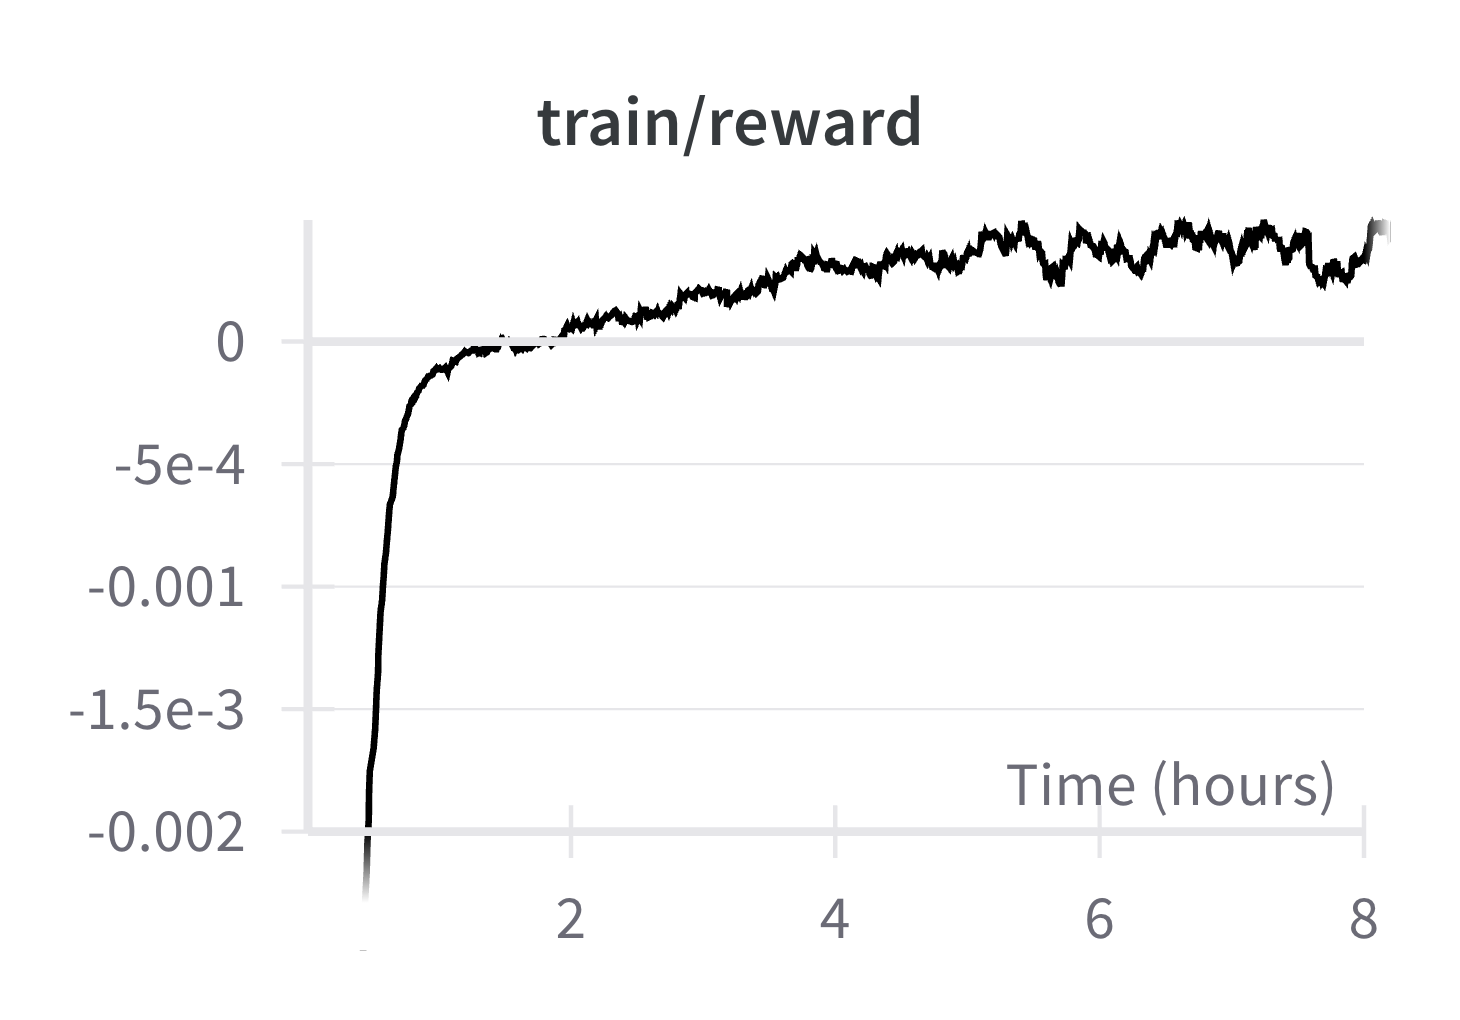
\includegraphics[width=0.4\linewidth]{figures/advection/training/train_reward.png}}
    \hfill
    \raisebox{-\height}{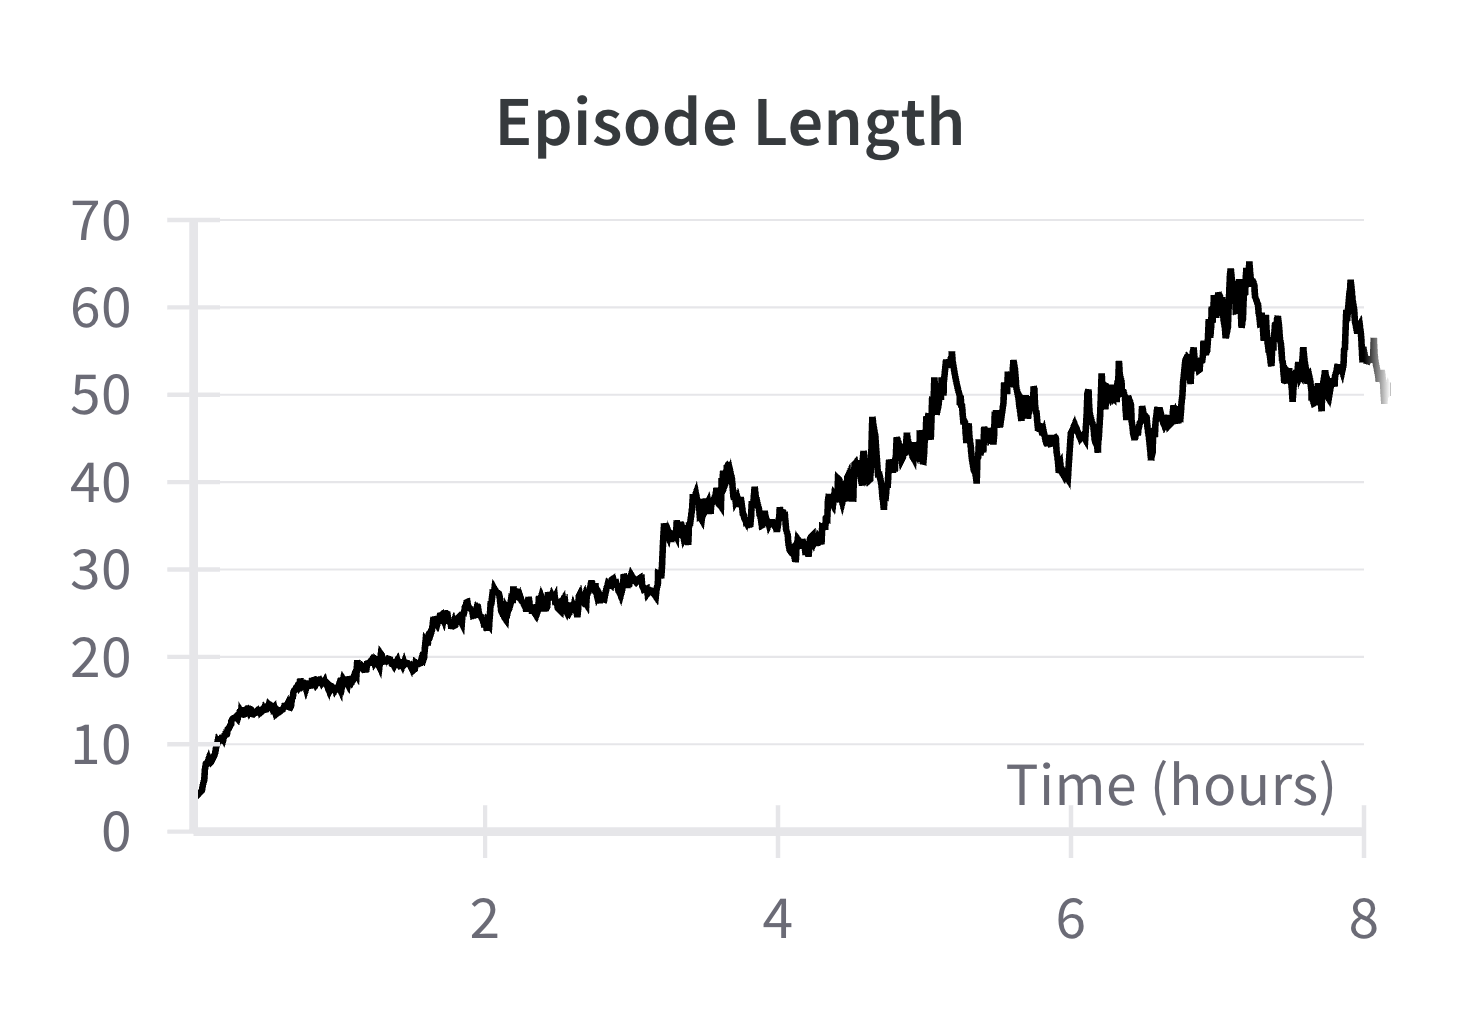
\includegraphics[width=0.4\linewidth]{figures/advection/training/train_length.png}}
    \hfill
    \caption{Visualizations of the evolution of the reward metric averaged over the agents and episode length during training on the advection equation.}
    \label{fig:advection_training_graphs}
\end{figure}

\begin{figure}[h]
    \centering
    \centering
    \hfill
    \raisebox{-\height}{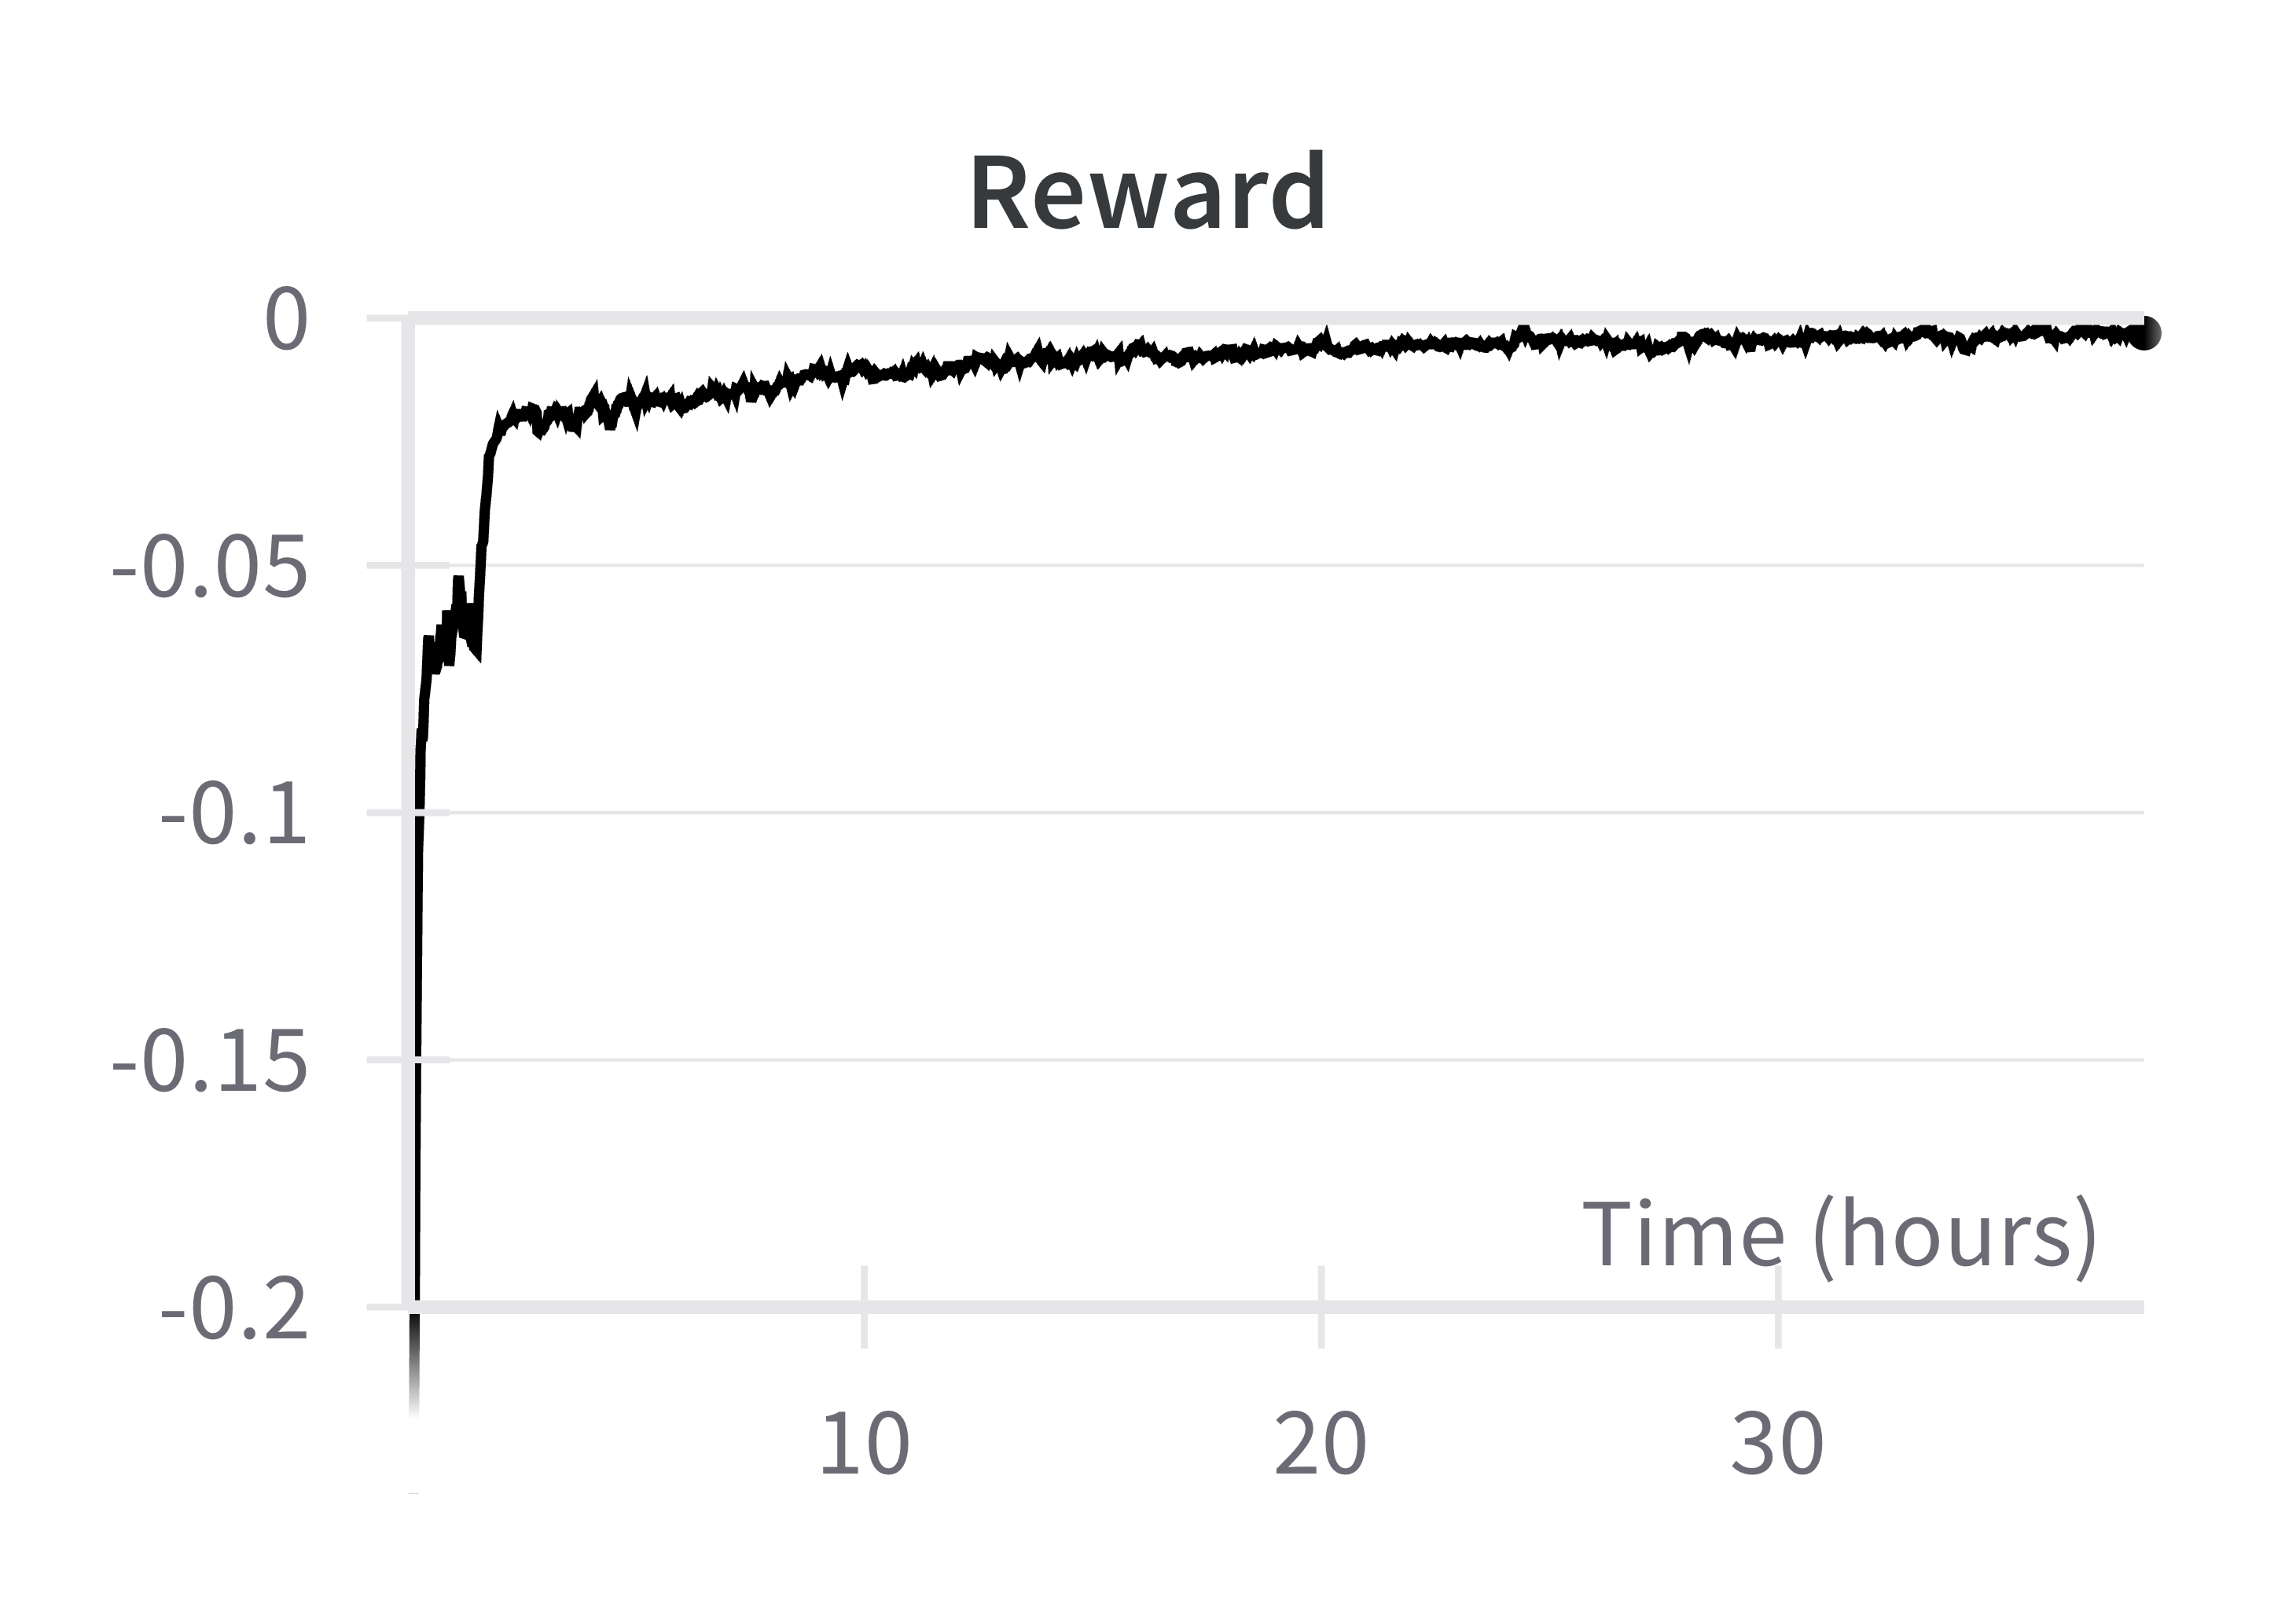
\includegraphics[width=0.4\linewidth]{figures/burgers/training/train_reward.png}}
    \hfill
    \raisebox{-\height}{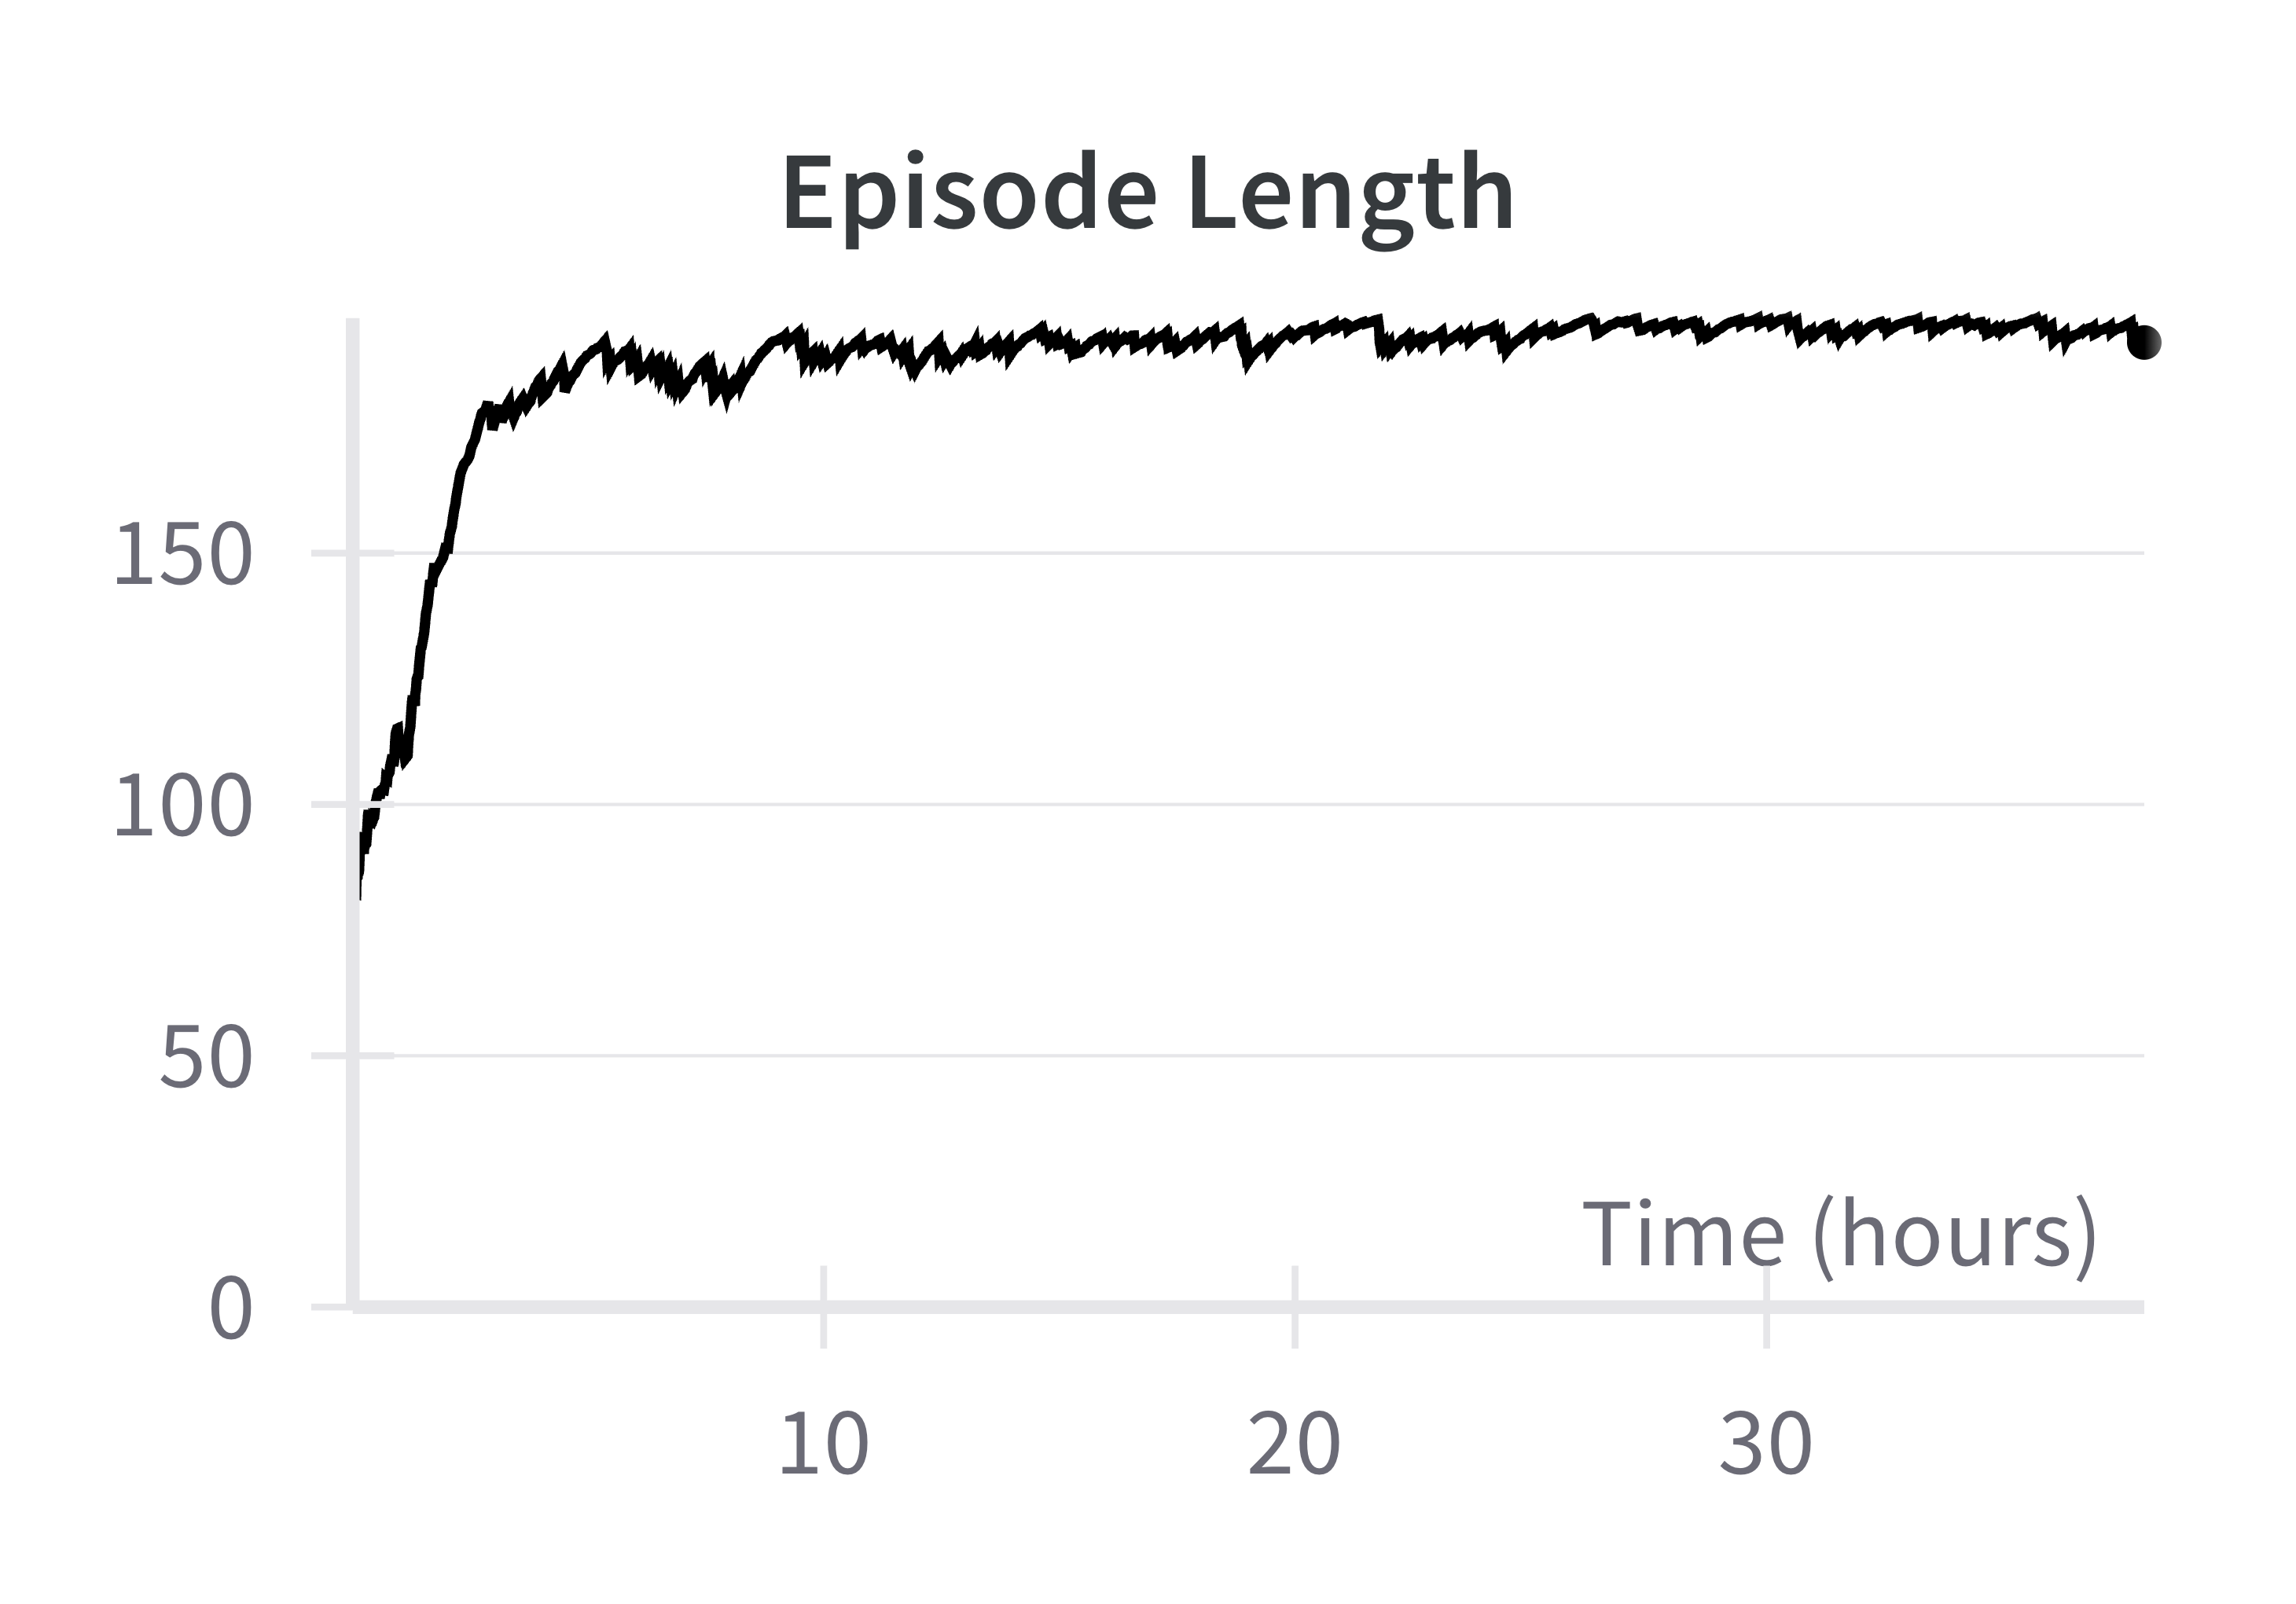
\includegraphics[width=0.4\linewidth]{figures/burgers/training/train_length.png}}
    \hfill
    \caption{Visualizations of the evolution of the reward metric averaged over the agents and episode length during training on the Burgers' equation.}
    \label{fig:burgers_training_graphs}
\end{figure}

\begin{table}[!ht]
\caption{Numerical values of the simulation parameters used for the advection CGS and FGS. Note that $\widetilde{\Delta t}$ is chosen to guarantee that the CFL condition in the CGS is fulfilled.}
\vskip 0.15in
\centering
\begin{tabular}{@{}l|c|l@{}}
\toprule
$\Omega$ & \multicolumn{2}{c}{$[0, 1] \times [0, 1]$} \\ 
$\tilde N_x$, $\tilde N_y$ & \multicolumn{2}{c}{64}  \\ 
$d, d_t$ &  \multicolumn{2}{c}{4}\\ 
\bottomrule
\multicolumn{3}{c}{Resulting other parameters:}  \\
\toprule
$ N_x$, $ N_y$ &   $d\cdot\tilde N_x,d\cdot \tilde N_y$ & $=256$ \\ 
$\Delta x, \Delta y$ &  $1/N_{x},1/N_y$ & $\approx 0,0039$  \\ 
$\widetilde{\Delta x}, \widetilde{\Delta y}$ &  $1/{\tilde N_{x}}, 1/{\tilde N_y}$ & $\approx 0,0156$   \\
$\widetilde{\Delta t}$ &  $0.9 \cdot \min(\widetilde{\Delta x}, \widetilde{\Delta y})$& $ \approx 0,0141$  \\
${\Delta t}$ &  $\widetilde{\Delta t}/{d_t}$  & $ \approx 0,0035$  \\ 
\bottomrule
\multicolumn{3}{c}{Discretization schemes:}  \\
\toprule
FGS, Space & \multicolumn{2}{c}{Central difference} \\
FGS, Time & \multicolumn{2}{c}{Fourth-order Runge-Kutta} \\
CGS, Space & \multicolumn{2}{c}{Upwind} \\
CGS, Time & \multicolumn{2}{c}{Forward Euler} \\
\bottomrule
\end{tabular}
\label{tab:advection_params}
\end{table}

\begin{table}[!ht]
\caption{Numerical values of the simulation parameters used for the Burgers' CGS and FGS. Again, $\widetilde{\Delta t}$ is chosen to guarantee that the CFL condition in the CGS is fulfilled.}
\vskip 0.15in
\centering
\begin{tabular}{@{}l|c|l@{}}
\toprule
$\Omega$ & \multicolumn{2}{c}{$[0, 1] \times [0, 1]$} \\ 
$\tilde N_x$, $\tilde N_y$ & \multicolumn{2}{c}{30}  \\ 
$d, d_t$ &  \multicolumn{2}{c}{5, 10}\\ 
\bottomrule
\multicolumn{3}{c}{Resulting other parameters:}  \\
\toprule
$ N_x$, $ N_y$ &   $d\cdot\tilde N_x,d\cdot \tilde N_y$ & $=150$ \\ 
$\Delta x, \Delta y$ &  $1/N_{x},1/N_y$ & $\approx 0,0067$  \\ 
$\widetilde{\Delta x}, \widetilde{\Delta y}$ &  $1/{\tilde N_{x}}, 1/{\tilde N_y}$ & $\approx 0,0333$   \\
$\widetilde{\Delta t}$ &  $0.9 \cdot \min(\widetilde{\Delta x}, \widetilde{\Delta y})$ & $ = 0,03$  \\
${\Delta t}$ &  $\widetilde{\Delta t}/{d_t}$ & $ = 0,003$  \\ 
\bottomrule
\multicolumn{3}{c}{Discretization schemes:}  \\
\toprule
FGS, Space & \multicolumn{2}{c}{Upwind} \\
FGS, Time & \multicolumn{2}{c}{Forward Euler} \\
CGS, Space & \multicolumn{2}{c}{Upwind} \\
CGS, Time & \multicolumn{2}{c}{Forward Euler} \\
\bottomrule
\end{tabular}
\label{tab:burgers_params}
\end{table}

\newpage
\subsection{Receptive Field of FCN}
In our CNN-MARL problem setting, the receptive field of the FCN corresponds to the observation $O_{ij}$ the agent at point $(i, j)$ is observing. In order to gain insight into this, we analyze the receptive field of our chosen architecture.

In the case of the given IRCNN architecture, the size of the receptive field (RF) of layer $i$ can be recursively calculated given the RF of layer afterward with
\begin{align}
    \text{RF}_{i+1} 
    &= \text{RF}_{i} + (\text{Kernel Size}_{i+1} - 1) \cdot \text{Dilation}_{i+1}\\
    &= \text{RF}_{i} + 2 \cdot \text{Dilation}_{i+1}.\\
\end{align}
The RF field of the first layer $\text{RF}_1$ is equal to its kernel size. By then using the recursive rule, we can calculate the RF at each layer and arrive at a value of $\text{RF}_7 = 33$ for the entire network. From this, we now arrive at the result that agent $(i,j)$ sees a $33 \times 33$ patch of the domain centered around its own location.
\begin{table}[h] 
\caption{Hyperparameters of each of the convolutional layers of the neural network architecture used for the advection equation experiment and the resulting receptive field (RF) at each layer. For the Burgers' equation experiment the architecture is simply adapted by setting the number of in channels of \texttt{Conv2D\_1} to 2 and the number of out channels of $\texttt{Conv2D}\_\pi$ to 4.} 
\vskip 0.15in
\centering
\begin{tabular}{|c|c|c|c|c|c|c|}
\hline
Layer & In Channels & Out Channels & Kernel & Padding & Dilation & RF \\
\hline
\texttt{Conv2D\_1} & 3 & 64 & 3 & 1 & 1 & 3\\
\hline
\texttt{Conv2D\_2} & 64 & 64 & 3 & 2 & 2 & 7 \\
\hline
\texttt{Conv2D\_3} & 64 & 64 & 3 & 3 & 3 & 13 \\
\hline
\texttt{Conv2D\_4} & 64 & 64 & 3 & 4 & 4 & 21 \\
\hline
\texttt{Conv2D\_5} & 64 & 64 & 3 & 3 & 3 & 27 \\
\hline
\texttt{Conv2D\_6} & 64 & 64 & 3 & 2 & 2 & 31 \\
\hline
\texttt{Conv2D}\_$\pi$ & 64 & 2 & 3 & 1 & 1 & 33 \\
\hline
\texttt{Conv2D}\_$\mathcal V$ & 64 & 1 & 3 & 1 & 1 & 33 \\
\hline
\end{tabular}
\label{tab:ircnn}
\end{table}

\subsection{Diverse Velocity Field Generation}
\subsubsection{Distribution for Training}\label{sec:train_vortices}
For the advection equation experiment, the velocity field is randomly generated by taking a linear combination of Taylor-Greene vortices and an additional random translational field. Let $\boldsymbol u_{ij}^{TG,k}, \boldsymbol v_{ij}^{TG,k}$ be the velocity components of the Taylor Greene Vortex with wave number $k$ that are defined as
\begin{align}
    \boldsymbol u_{ij}^{TG,k} &:= \cos(k\boldsymbol x_{i}) \cdot \sin(k \boldsymbol y_j) \\
    \boldsymbol v_{ij}^{TG,k} &:= - \sin(k\boldsymbol x_i) \cdot \cos(k\boldsymbol y_h).
\end{align}
Furthermore, define the velocity components of a translational velocity field as $u^{TL}, v^{TL} \in \mathbb R$. To generate a random incompressible velocity field, we sample 1 to 4 $k$'s from the set $\{1, ..., 6\}$.
For each $k$, we also sample a $\text{sign}_k$ uniformly from the set $\{-1, 1\}$ in order to randomize the vortex directions. For an additional translation term, we sample $u^{TL}, v^{TL}$ independently from  $\text{uniform}(-1, 1)$. We then initialize the velocity field to
\begin{align}
    \boldsymbol u_{ij} &:= u^{TL} + \sum_k \text{sign}_k \cdot \boldsymbol u_{ij}^{TG,k}\\
    \boldsymbol v_{ij} &:= v^{TL} + \sum_k \text{sign}_k \cdot \boldsymbol v_{ij}^{TG,k}.
\end{align}
We will refer to this distribution of vortices as $\mathcal D^{Vortex}_{Train}$. 

For the Burgers' equation experiment, we make some minor modifications to the sampling procedure. The sampling of translational velocity components is omitted and $2$ to $4$ $k$'s are sampled from $\{2, 4, 6, 8\}$. The latter ensures that the periodic boundary conditions are fulfilled during initialization which is important for the stability of the simulations.

\subsubsection{Distribution for Testing} \label{sec:test_vortices}
First, a random sign \( \text{sign} \) is sampled from the set \(\{-1, 1\}\). Subsequently, a scalar \( a\) is randomly sampled from a uniform distribution bounded between 0.5 and 1. The randomization modulates both the magnitude of the velocity components and the direction of the vortex, effectively making the field random yet structured. The functional forms of \(\boldsymbol u_{ij}^{C}\) and \(\boldsymbol v_{ij}^{C}\) are then expressed as
\begin{align}
    \boldsymbol u_{ij}^{V} &:= \text{sign} \cdot  a \cdot \sin^2(\pi \boldsymbol x_i) \sin(2\pi \boldsymbol y_j) \\
    \boldsymbol v_{ij}^{V} &:= - \text{sign} \cdot a \cdot\sin^2(\pi \boldsymbol y_j) \sin(2\pi \boldsymbol x_i).
\end{align}
In the further discussion, we will refer to this distribution of vortices as $\mathcal D^{Vortex}_{Test}$.

\subsection{Computational Complexity}
To quantitatively compare the execution times of the different simulations, we measure the runtime of performing one update step of the environment and report them in \cref{tab:execution_times}. As expected, CNN-MARL increases the runtime of the CGS. However, it stays below the FGS times by at least a factor of $5$. The difference is especially pronounced in the example of the advection equation, where the FGS uses a high order scheme on a fine grid, which leads to an execution time difference between CNN-MARL and FGS of more than an order of magnitude.
\begin{table}[t] 
\caption{Runtime of one simulation step in ms of the different simulations averaged over 500 steps.}
\label{tab:execution_times}
\vskip 0.15in
\begin{center}
\begin{scriptsize}
\begin{sc}
\begin{tabular}{l|cccr}
\toprule
 & CGS & ACGS & CNN-MARL & FGS \\
\midrule
Advection    & $\tiny 0.31 \pm 0.00$& $\tiny 0.96 \pm 0.00$& $\tiny 2.66 \pm 0.96$ & $\tiny 89.52 \pm 0.47$ \\
Burgers' & $\tiny 0.25 \pm 0.00$ & -& $\tiny 1.82 \pm 0.01$ & $\tiny 10.16 \pm 0.03$\\
\bottomrule
\end{tabular}
\end{sc}
\end{scriptsize}
\end{center}
\vskip -0.1in
\end{table}

\newpage
\section{Proof: Theoretically Optimal Action} \label{sec:proof_optimal_action}
To explore how the actions of the agents can be interpreted, we analyze the optimal actions based on the used numerical schemes. The \textit{perfect} solution would fulfill 
$$
 \mathcal{M}( \tilde{\boldsymbol \psi^n}) +\tilde{ \boldsymbol \epsilon^n}  = 0.
$$

Here, $\mathcal{M}$ is the numerical approximation of the PDE an  $\tilde{\boldsymbol \epsilon^n}$ is the truncation error.

We refer to the numerical approximations of the derivatives in the CGS as $\mathcal{T}^{FE}$ for forward Euler and $\mathcal{D}^{UW}$ for the upwind scheme. We obtain
\begin{align}
    0 &=  \mathcal{M}(\tilde{\boldsymbol\psi^n})+ \tilde{\boldsymbol\epsilon}^n\\
     &=\mathcal{T}^{FE}(\tilde{\boldsymbol\psi}^n, \tilde{\boldsymbol\psi}^{n+1}) + \tilde{\boldsymbol u}^n \mathcal{D}^{UW}_x(\tilde{\boldsymbol\psi}^n) + \tilde{\boldsymbol v}^n \mathcal{D}^{UW}_y(\tilde{\boldsymbol\psi}^n) + \tilde{\boldsymbol\epsilon}^n \\
     &=\frac{\tilde{\boldsymbol\psi}^{n+1} - \tilde{\boldsymbol\psi}^n}{\widetilde{\Delta t}} + \tilde{\boldsymbol u}^n \mathcal{D}^{UW}_x(\tilde{\boldsymbol\psi}^n) + \tilde{\boldsymbol v}^n \mathcal{D}^{UW}_y(\tilde{\boldsymbol\psi}^n) + \tilde{\boldsymbol\epsilon}^n. \\
\end{align}


By rewriting, we obtain the following time stepping rule
\begin{align}
   \tilde{\boldsymbol\psi}^{n+1} 
   &= \tilde{\boldsymbol\psi}^n - \widetilde{\Delta t} \left(\tilde{\boldsymbol u}^n \mathcal{D}^{UW}_x(\tilde{\boldsymbol\psi}^n) + \tilde{\boldsymbol v}^n \mathcal{D}^{UW}_y(\tilde{\boldsymbol\psi}^n) + \tilde{\boldsymbol\epsilon}^n\right)\\
   &= \tilde{\boldsymbol\psi}^n - \widetilde{\Delta t} \left(\tilde{\boldsymbol u}^n \mathcal{D}^{UW}_x(\tilde{\boldsymbol\psi}^n) + \tilde{\boldsymbol v}^n \mathcal{D}^{UW}_y(\tilde{\boldsymbol\psi}^n)\right) - \widetilde{\Delta t} \tilde{\boldsymbol \epsilon}^n\\
   &= \mathcal G(\tilde{\boldsymbol\psi}^n, \tilde C^n) - \widetilde{\Delta t} \tilde{\boldsymbol\epsilon}^n.
\end{align}

where $\tilde C^n:=(\tilde{\boldsymbol u}^n, \tilde{\boldsymbol v}^n)$. This update rule would theoretically find the \textit{exact} solution. It involves a coarse step followed by an additive correction after each step. We can define $ \tilde{\boldsymbol\phi}^{n+1} :=\tilde{\boldsymbol\psi}^{n+1} + \widetilde{\Delta t} \tilde{\boldsymbol\epsilon}^n$, to bring the equation into the same form as seen in the definition of the RL environment
$$ 
\tilde{\boldsymbol\phi}^{n+1} = \mathcal G(\tilde{\boldsymbol\phi}^{n} - \widetilde{\Delta t} \tilde{\boldsymbol\epsilon}^{n-1}, \tilde C^n),
$$
which illustrates that the optimal action at step $n$ would be the previous truncation error times the time increment
\begin{equation}
    \boxed{
    {\boldsymbol A^n}^* = \widetilde{\Delta t} \tilde{\boldsymbol\epsilon}^{n-1}.
    }
\end{equation}

%%%%%%%%%%%%%%%%%%%%%%%%%%%%%%%%%%%%%%%%%%%%%%%%%%%%%%%%%%%%%%%%%%%%%%%%%%%%%%%
%%%%%%%%%%%%%%%%%%%%%%%%%%%%%%%%%%%%%%%%%%%%%%%%%%%%%%%%%%%%%%%%%%%%%%%%%%%%%%%


\end{document}


% This document was modified from the file originally made available by
% Pat Langley and Andrea Danyluk for ICML-2K. This version was created
% by Iain Murray in 2018, and modified by Alexandre Bouchard in
% 2019 and 2021 and by Csaba Szepesvari, Gang Niu and Sivan Sabato in 2022.
% Modified again in 2023 by Sivan Sabato and Jonathan Scarlett.
% Previous contributors include Dan Roy, Lise Getoor and Tobias
% Scheffer, which was slightly modified from the 2010 version by
% Thorsten Joachims & Johannes Fuernkranz, slightly modified from the
% 2009 version by Kiri Wagstaff and Sam Roweis's 2008 version, which is
% slightly modified from Prasad Tadepalli's 2007 version which is a
% lightly changed version of the previous year's version by Andrew
% Moore, which was in turn edited from those of Kristian Kersting and
% Codrina Lauth. Alex Smola contributed to the algorithmic style files.
